\documentclass[xetex, onlymath, aspectratio=169]{beamer}
\usefonttheme{serif}
\usetheme{hsr}

% use lmodern for math
\usepackage{lmodern}

% math packages
\usepackage{amsmath}
\usepackage{amssymb}
\usepackage{bm}
\usepackage{cancel}
\renewcommand{\CancelColor}{\color{red}}

\renewcommand{\vec}[1]{\mathbf{\bm{#1}}}

% use plex font for monospaced, roboto for the rest
\usepackage[T1]{fontenc}
\usepackage{plex-otf} % monospaced
% \usepackage{roboto} % other
\renewcommand*\familydefault{\sfdefault}

\usepackage{graphicx}
\usepackage{booktabs}
\usepackage{array}

% biblopgraphy
\usepackage[backend=bibtex, style=ieee]{biblatex}
\addbibresource{KugelBSc.bib}

% links
\usepackage{hyperref}
\hypersetup{
  % Remove ugly boxes
  hidelinks,
  % Set colors
  colorlinks = true,
  anchorcolor = black,
  citecolor = black,
  filecolor = black,
  linkcolor = black,
  menucolor = black,
  runcolor = black,
  urlcolor = {black!50!blue}, 
}

% pretty drawings
\usepackage{tikz}
\usetikzlibrary{calc}
\usepackage{xcolor}
\usepackage{pgfplots}
\pgfplotsset{compat=1.9}

% source code
\usepackage{listings}
%% create a lstlisting style
\lstdefinestyle{samplestyle}{
  belowcaptionskip=\baselineskip,
  breaklines=true,
  frame=none,
  inputencoding=utf8,
  % margin
  xleftmargin=\parindent,
  % background
  backgroundcolor=\color{hsr-lightgrey20},
  % default language:
  language=[LaTeX]TeX,
  showstringspaces=false,
  % font
  basicstyle=\ttfamily\small,
  identifierstyle=\color{hsr-black},
  keywordstyle=\color{hsr-blue},
  commentstyle=\color{hsr-black40},
  stringstyle=\color{hsr-mauve80},
}

%% and set the chosen style
\lstset{style=samplestyle, escapechar=`}

% metadata
\title{Spherical Harmonics}
\author[NaoPross]{\texttt{Naoki Pross, Manuel Cattaneo}}
\date{Spring Semester 2022}

\institute[OST]{OST FHO Campus Rapperswil}
% \logo{\includegraphics[width=3cm]{figs/hsr-logo}}

\AtBeginSection[]
{
  \begin{frame}
    \frametitle{Table of Contents}
    \tableofcontents[currentsection]
  \end{frame}
}


\begin{document}

\frame{
  \maketitle
}

\begin{frame}{Goals for Today}
	\Large \uncover<1->{\textbf{Spherical Harmonics}} \uncover<2->{\,\textit{and}\, \textbf{Electron Orbitals}}
	\begin{tikzpicture}
  	\uncover<1->{
			\node (i1) {
      	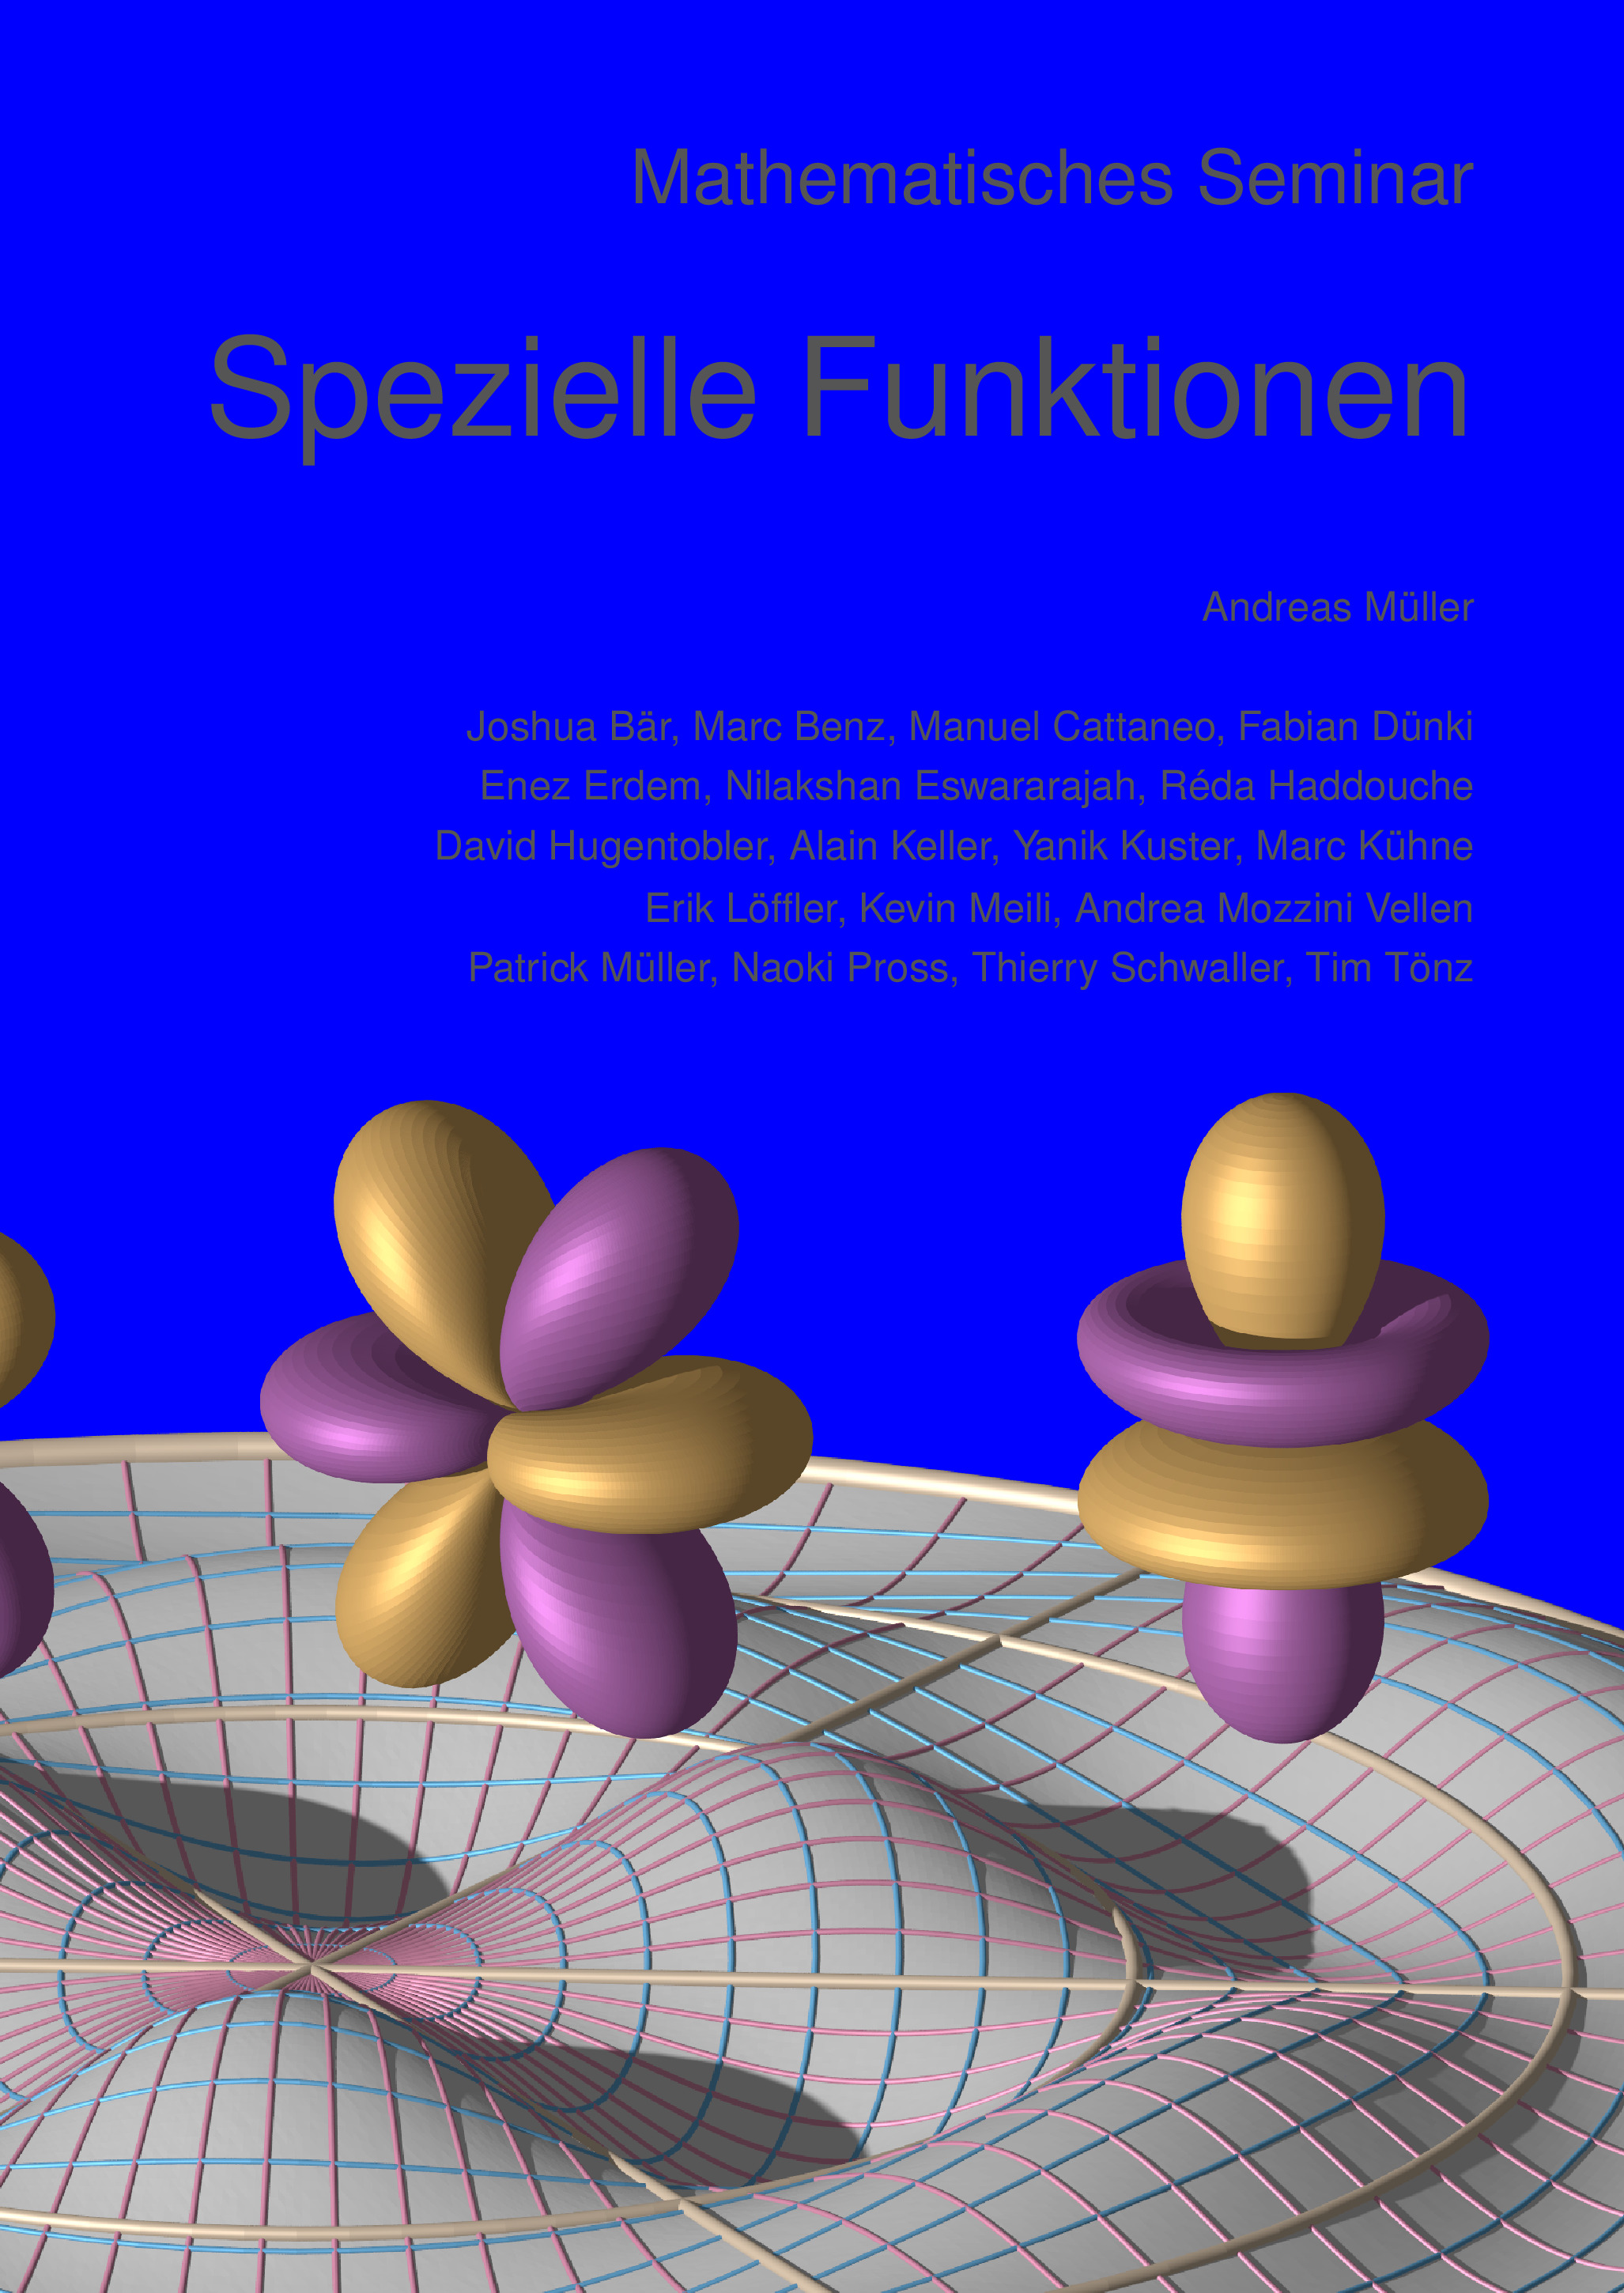
\includegraphics[height=8cm, trim=200 100 50 50, clip]{figures/buchcover}
			};
  	}
  
  	\uncover<2->{
  		\node (i2) at ($(i1) + (2cm, 0)$) {
				\nocite{minutephysics_better_2021}
  			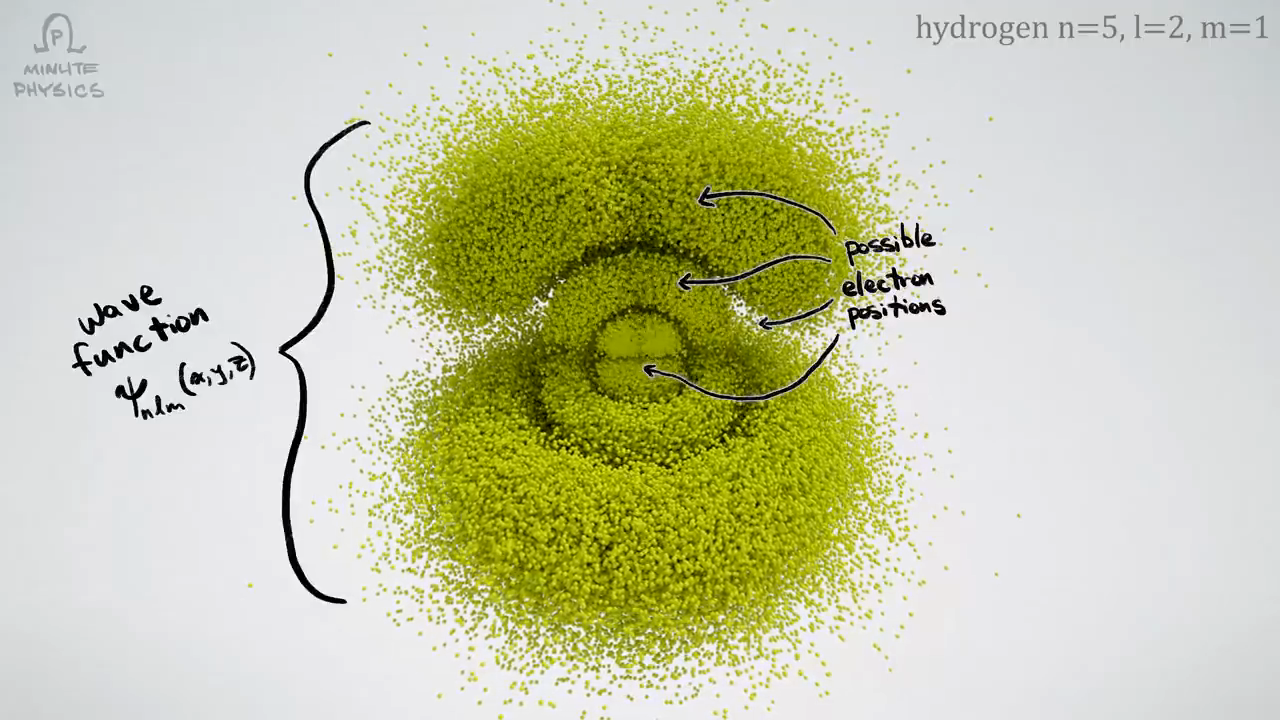
\includegraphics[height=65mm]{figures/orbitals-minutephysics}
  		};
  	}
	\end{tikzpicture}
\end{frame}

\frame{
  \frametitle{Table of Contents}
	\tableofcontents
}

\section{Fourier on \(\mathbb{R}^2\)}

\begin{frame}{Nice Periodic Functions}
	\begin{columns}
		\begin{column}{.7\linewidth}
    	\begin{definition}
    		A function
    		\[
    			f : \mathbb{R}^2 \to \mathbb{C}
    		\]
    		is a ``nice periodic function'' when it is
    		\begin{itemize}
    			\item smooth,
    			\item differentiable,
    			\item \textcolor{gray}{(abs.)} integrable,
    			\item periodic on \([0, 1] \times [0, 1]\), i.e.
    				\[
    					f(\xi, \eta) = f(\xi + 1, \eta) = f(\xi, \eta + 1).
    				\]
    		\end{itemize}
    	\end{definition}
		\end{column}
		\begin{column}{.3\linewidth}
			\begin{center}
				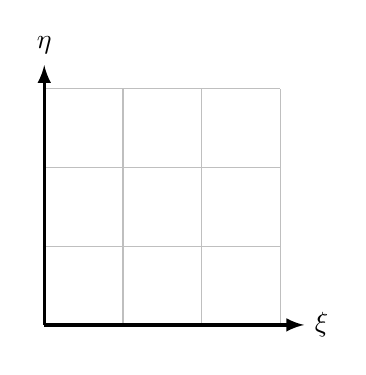
\begin{tikzpicture}[
					axis/.style = {
						very thick, -latex, draw = black
					},
				]
					\draw[lightgray] (0, 0) grid (3, 3);
					\draw[axis] (0, 0) -- (3.3, 0) node[right] {\(\xi\)};
					\draw[axis] (0, 0) -- (0, 3.3) node[above] {\(\eta\)};
				\end{tikzpicture}
			\end{center}
		\end{column}
	\end{columns}		
\end{frame}

\begin{frame}{Function Space}
	\begin{block}{Basis Functions}
  	The space of nice periodic functions is spanned by the (also nice) functions
  	\[
  		B_{m, n}(\xi, \eta) = e^{i2\pi m\xi} e^{i2\pi n\eta}.
  	\]
	\end{block}
\end{frame}

\begin{frame} \centering
	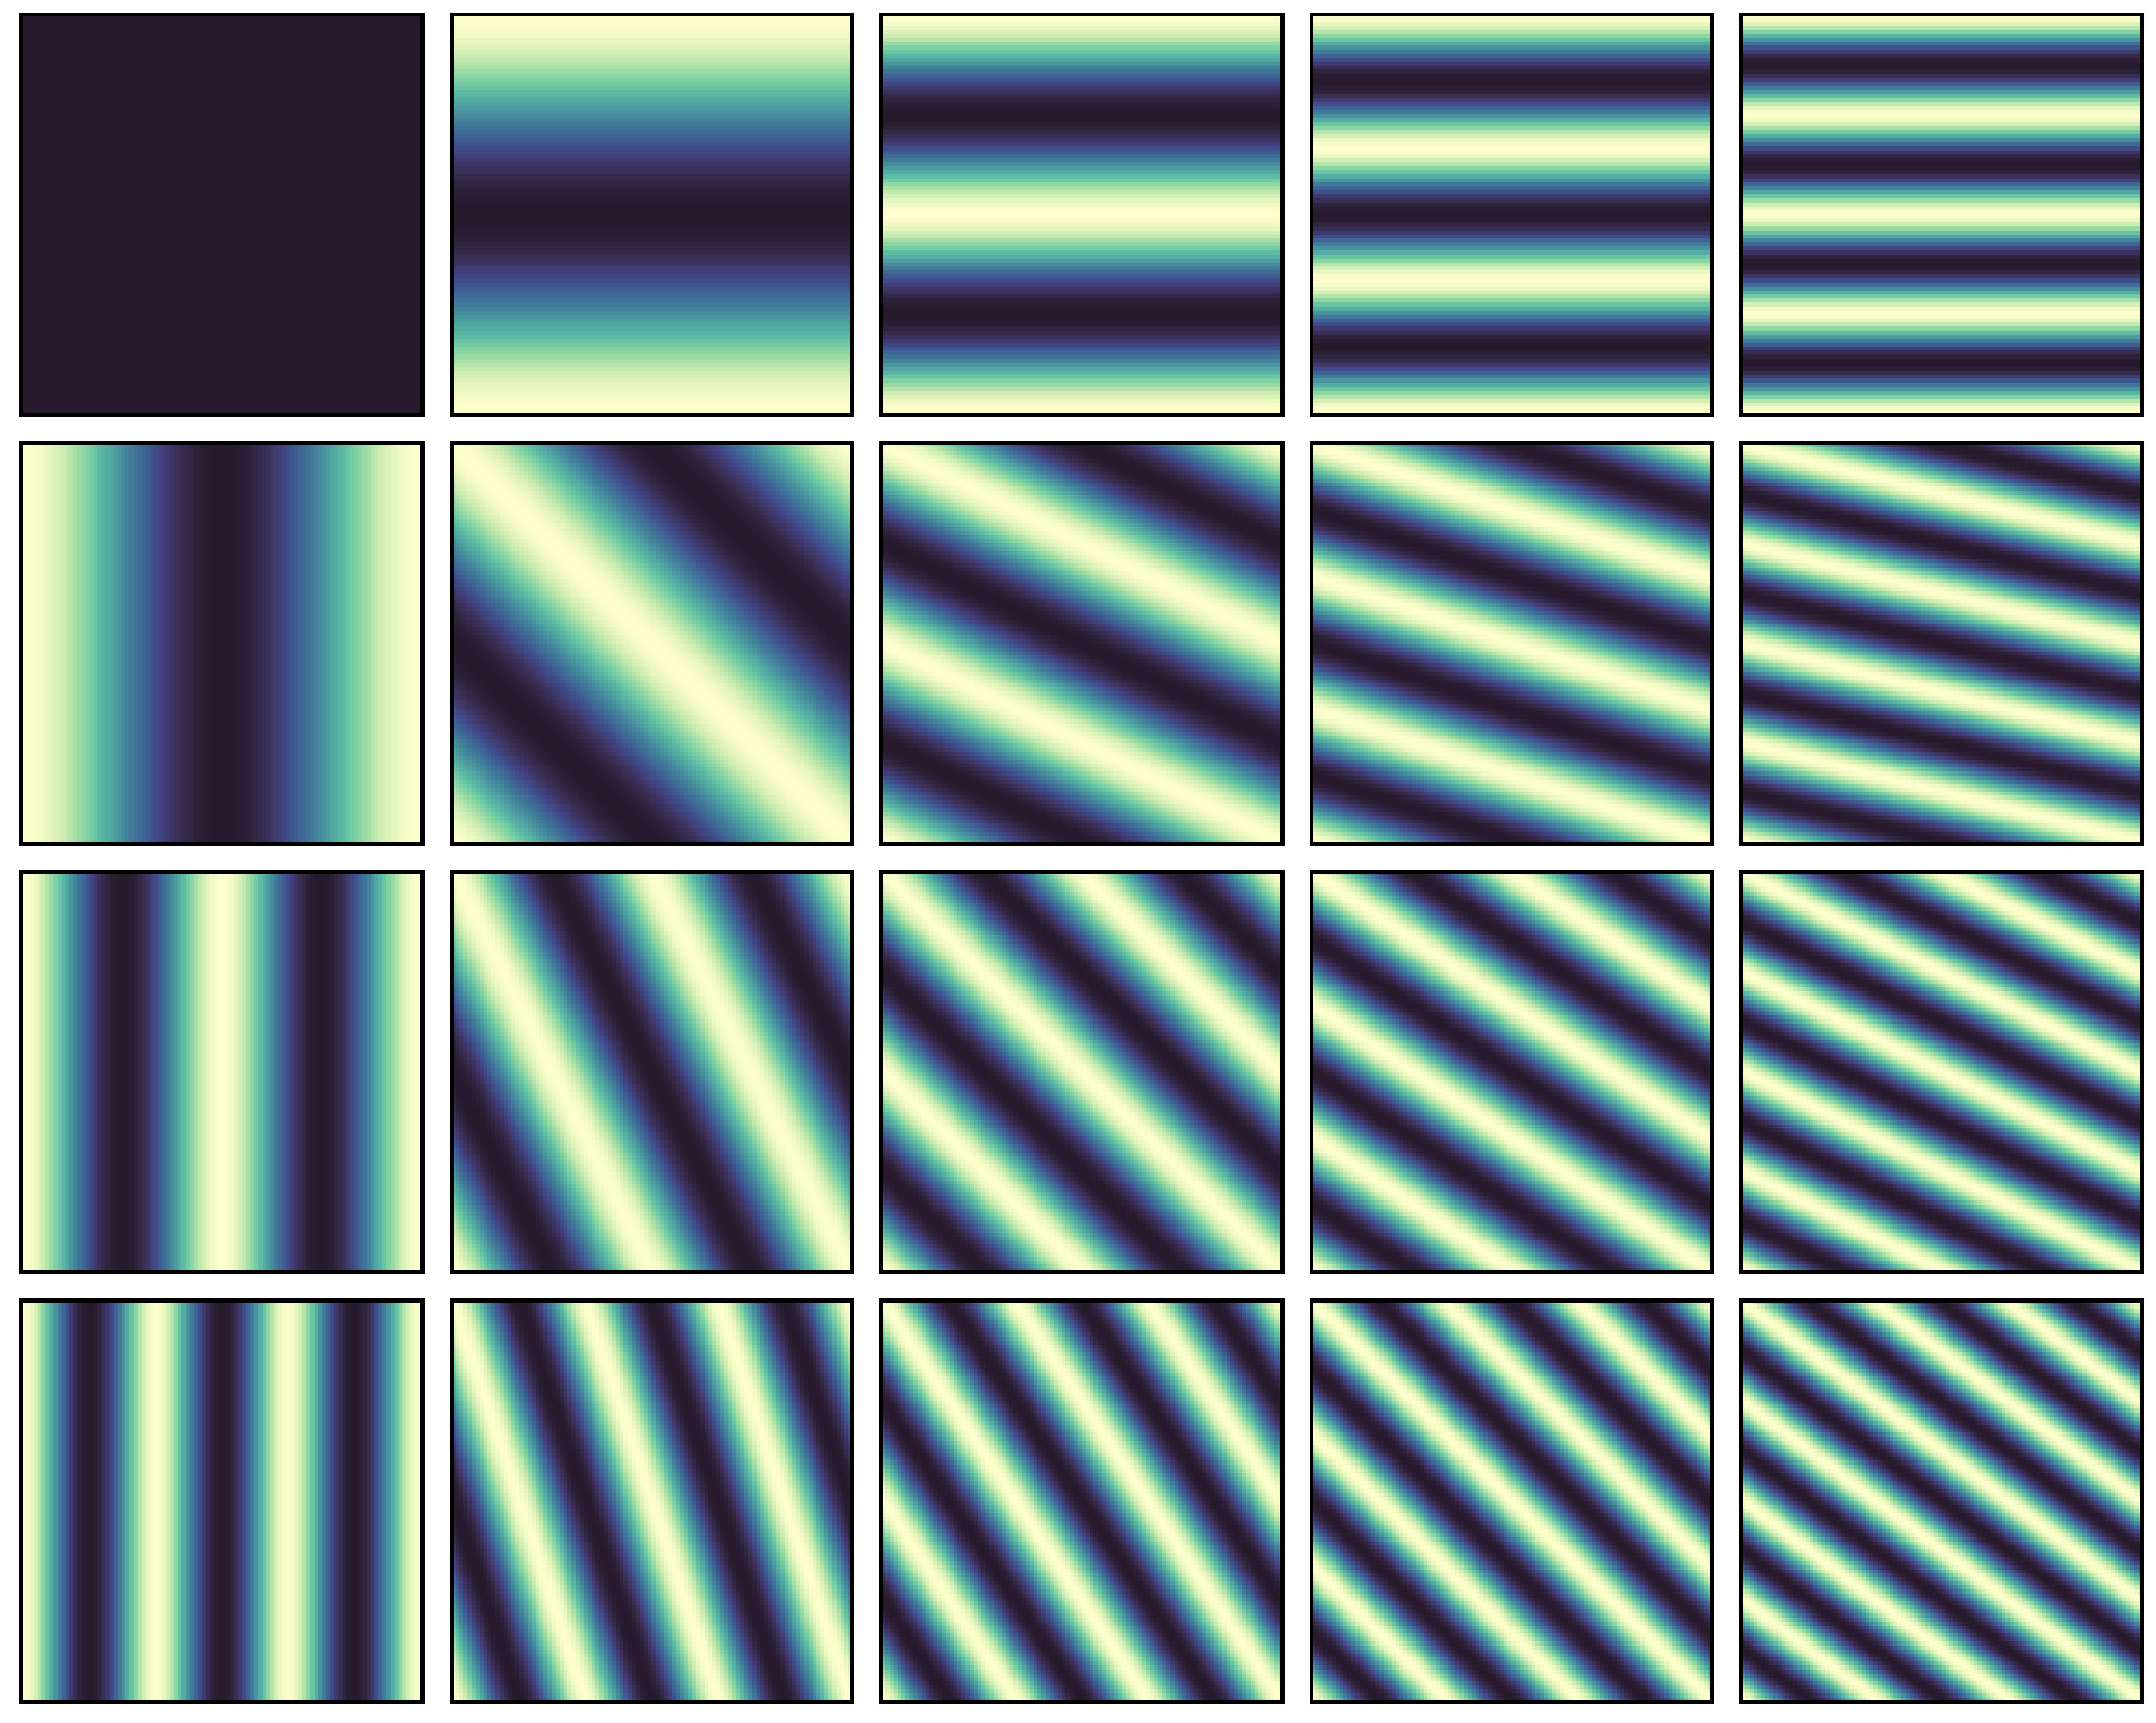
\includegraphics[height=.9\paperheight]{figures/flat-basis-functions}
\end{frame}

\begin{frame}{Inner Product}
	\begin{definition}<1->
		Let \(f(\xi, \eta)\) and \(g(\xi, \eta)\) be nice periodic functions. Their inner product is
		\[
			\langle f, g \rangle = \iint_{[0, 1]^2} f(\xi, \eta) \overline{g}(\xi, \eta) \, d\xi d\eta.
		\]
	\end{definition}

	\begin{definition}<2->
		For a nice periodic function \(f(\xi, \eta)\): the numbers
		\[
			c_{m, n} = \langle f, B_{m, n} \rangle
		\]
		are the \emph{Fourier coefficients} or \emph{spectrum} of \(f\). 
	\end{definition}
\end{frame}

\begin{frame}{Fourier Series}
	\begin{theorem}
		For nice periodic functions:
  	\[
  		f(\xi, \eta) = \sum_{m \in \mathbb{Z}} \sum_{n \in \mathbb{Z}}
				c_{m, n} B_{m, n} (\xi, \eta)
  	\]
		where
		\[
			c_{m, n} = \langle f, B_{m, n} \rangle.
		\]
	\end{theorem}
\end{frame}

\begin{frame}{Why exponentials?}
	
	\centering

	{\huge\bfseries\itshape Why \(B_{m, n} = e^{i2\pi m\xi} e^{i2\pi n\eta}\)?}
	\vspace{3em}
	
	{\huge\bfseries\itshape Because
		{\Huge \(\nabla^2\)}
	}
	
\end{frame}

\begin{frame}{The Problem}
	\begin{block}{Eigenvalue Problem}<1->
		\[
			\nabla^2 f(\xi, \eta)
			  = \frac{\partial^2 f}{\partial \xi^2} + \frac{\partial^2 f}{\partial \eta^2}
			  = \lambda f(\xi, \eta)
		\]
	\end{block}
	\begin{alertblock}{Solution}<2->
		Separation ansatz:
		\[
			f(\xi, \eta) = M(\xi) N(\eta)
		\]
		Resulting ODEs:
		\begin{align*}
			\frac{d^2 M}{d \xi^2} &= \kappa M(\xi), & \frac{d^2 N}{d \eta^2} &= (\lambda - \kappa) N(\eta)
		\end{align*}
	\end{alertblock}
\end{frame}

\section{The functions \(Y_{m, n}(\varphi, \vartheta)\)}

\begin{frame}{Spherical Coordinates}
	\begin{columns}
		\begin{column}{.6\linewidth}
			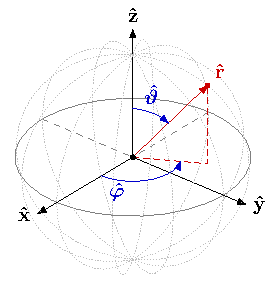
\includegraphics[height=.9\paperheight]{figures/spherical-coordinates}
		\end{column}
		\begin{column}{.4\linewidth}
			\noindent
			Variables
			\begin{align*}
				r &\in \mathbb{R}^+ \\
				\vartheta &\in [0, \pi] \\
				\varphi &\in [0, 2\pi)
			\end{align*}
			To cartesian
			\begin{align*}
				x &= r\cos\varphi \sin\vartheta \\
				y &= r\sin\varphi\sin\vartheta \\
				z &= r\cos\vartheta
			\end{align*}
		\end{column}
	\end{columns}
\end{frame}

\begin{frame}{Spherical Laplacian}
	\uncover<1->{
  	Cartesian Laplacian
  	\[
  		\nabla^2 := \frac{\partial^2}{\partial \xi^2} + \frac{\partial^2}{\partial \eta^2}
  	\]
	}
	
	\uncover<2->{
  	Spherical Laplacian
  	\[
  		\nabla^2 :=
  			\frac{1}{r^2} \frac{\partial}{\partial r} \left( r^2 \frac{\partial}{\partial r} \right)
    			+ \frac{1}{r^2} \onslide<3-> \underbrace{ \onslide<2-> \left[
  						\frac{1}{\sin\vartheta} \frac{\partial}{\partial \vartheta}
  						\left( \sin\vartheta \frac{\partial}{\partial\vartheta} \right)
  						+ \frac{1}{\sin^2 \vartheta} \frac{\partial^2}{\partial\varphi^2}
  					\right]
  				\onslide<3-> }_{\text{Surface Spherical Laplacian}~ \nabla^2_s} \onslide<2->
  	\]
	}
	
	\uncover<4->{
  	Surface Spherical Laplacian
  	\[
  		\nabla^2_s := r^2 \nabla^2
  			- \frac{\partial}{\partial r} \left( r^2 \frac{\partial}{\partial r} \right)
  	\]
	}
\end{frame}

\begin{frame}[fragile]{Geometrical Intuition}
	\only<1>{
		\begin{center}
  		\begin{tikzpicture}
				\begin{axis}[
					clip = false,
					width = .8\linewidth, height = .8\paperheight,
					xtick = \empty, ytick = \empty,
					colormap name = viridis,
					axis lines = middle,
					axis line style = {ultra thick, -latex}
				]
        	\addplot+[
						smooth, mark=none, line width = 3pt, mesh,
						point meta=explicit,
					] file {figures/laplacian-1d.dat};
        \end{axis}
  		\end{tikzpicture}
		\end{center}
	}
	\only<2>{
		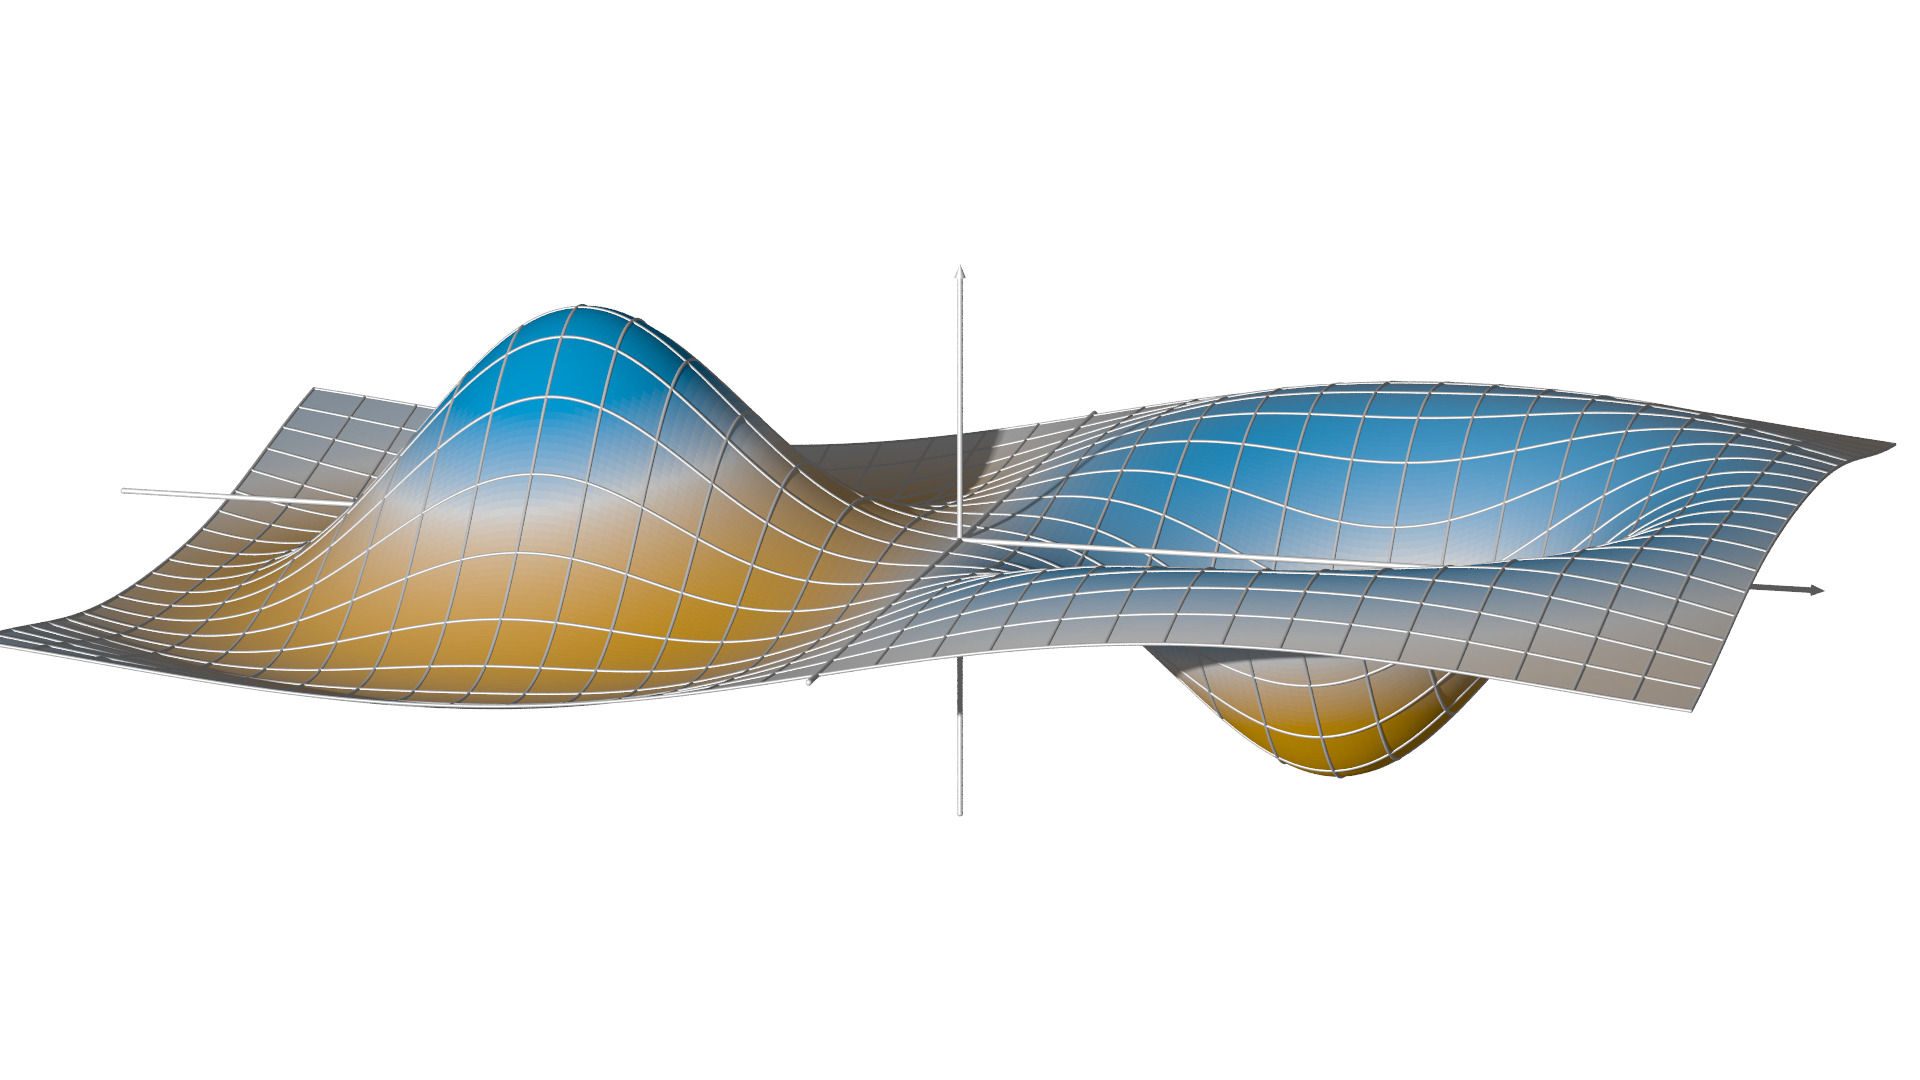
\includegraphics[width=\linewidth]{figures/laplacian-3d}
	}
	\only<3>{
		\begin{center}
			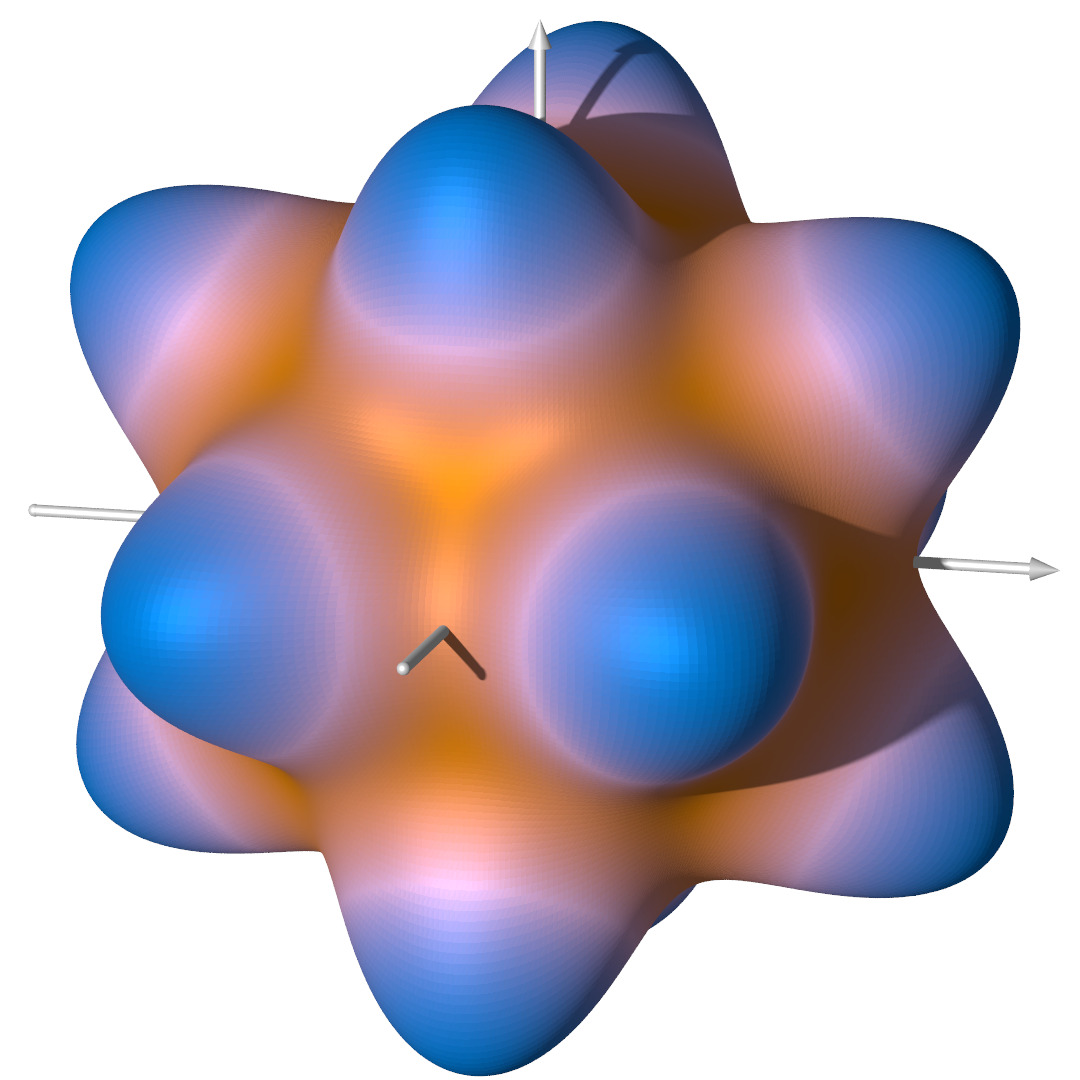
\includegraphics[height=.7\paperheight]{figures/laplacian-sphere}
		\end{center}
	}
\end{frame}

\begin{frame}{Where is \(\nabla^2_s\) useful?}
	To do brain scans, apparently \cite{carvalhaes_surface_2015}
		\begin{center}
		\only<1>{
			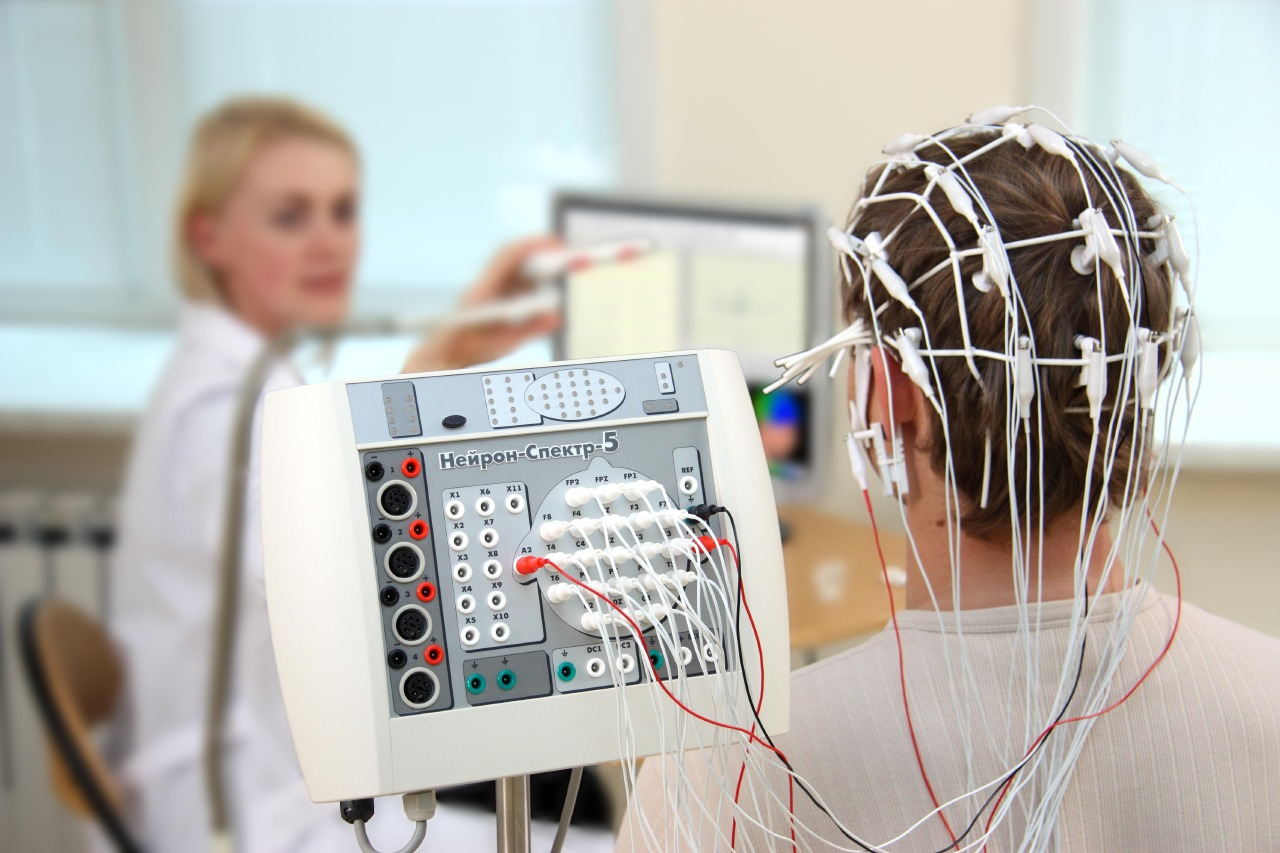
\includegraphics[width=.8\linewidth, clip, trim=0 20 0 20]{figures/eeg-photo}
			\nocite{baburov__2009}
			% \caption{Electroencephalogram (EEG). Image from Wikimedia \cite{baburov__2009}.}
		}
		\only<2>{
    	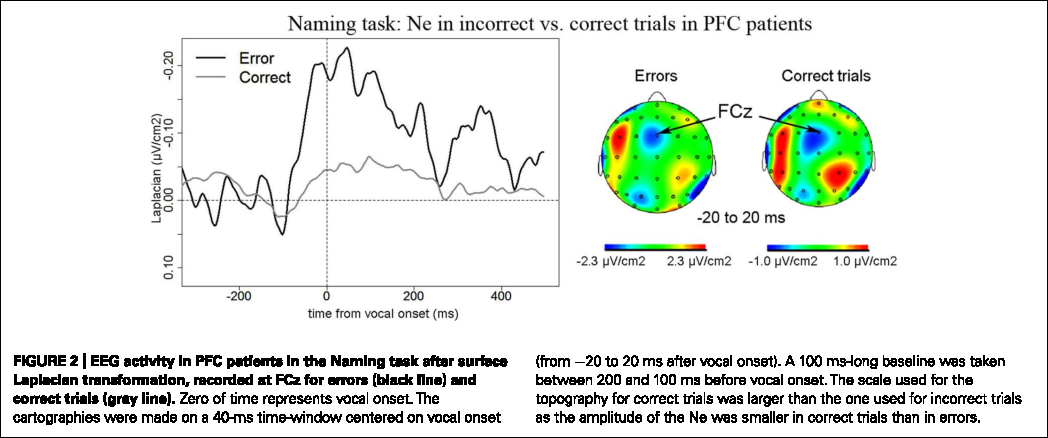
\includegraphics[width=\linewidth]{figures/surface-laplacian-eeg}
			\nocite{ries_role_2013}
    	% \caption{Surface Laplacian in EEG. Taken from \cite{ries_role_2013}.}
		}
	\end{center}
\end{frame}

\begin{frame}{Brain Scans}
	\begin{columns}
		\begin{column}{.6\linewidth}
    	Electrodynamics
    	\begin{align*}
	    	\onslide<1->{
					\nabla^2 \phi &= \bm{\nabla \cdot} \bm{\nabla} \phi \qquad
						\color{lightgray} \left(
						\phi = \int_\mathsf{A}^\mathsf{B} \vec{E} \bm{\cdot} d\vec{l}
					\right) \\
				}
				\onslide<2->{
					&= \bm{\nabla \cdot} \vec{E} \\
				}
				\onslide<3->{
		  		&\color{lightgray}= \int_{\Omega} (\bm{\nabla \cdot} \vec{E}) \bm{\cdot} d\vec{s}
		   		= \oint_{\partial \Omega} \vec{E} \bm{\cdot} d\vec{s} \\
				}
				\onslide<4->{
					&= \frac{\rho}{\varepsilon}
				}
    	\end{align*}
			\uncover<5->{
      	So over the scalp
      	\[
      		\nabla^2_s \phi
      			= \frac{\rho_s}{\varepsilon}
      			= \text{Current flow in the brain}
      	\]
			}
		\end{column}
		\begin{column}{.4\linewidth}
			\uncover<2->{
  			\centering
  			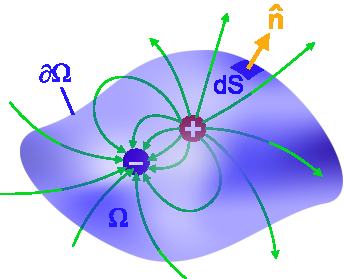
\includegraphics[width=\linewidth]{figures/flux}
  			\nocite{maschen_divergence_2013}
			}
		\end{column}
	\end{columns}
\end{frame}

\begin{frame}{New Hard Problem}
	\begin{block}{The Problem}<1->
		\only<1>{
			\[
				\nabla^2_s f(\varphi, \vartheta) = \lambda f(\varphi, \vartheta)
			\]
		}
		\only<2->{
			\[
  			\frac{1}{\sin\vartheta} \frac{\partial}{\partial \vartheta}
  					\left( \sin\vartheta \frac{\partial f}{\partial\vartheta} \right)
  					+ \frac{1}{\sin^2 \vartheta} \frac{\partial^2 f}{\partial\varphi^2}
  				= \lambda f(\varphi, \vartheta)
			\]
		}
	\end{block}
	\begin{alertblock}{Idea}<3->
		Separation ansatz:
		\[
			f(\varphi, \vartheta) = \Phi(\varphi) \Theta(\vartheta)
		\]
		From the ``easy'' part:
		\[
			\frac{d^2\Phi}{d\varphi^2} = \kappa \Phi(\varphi)
				\implies \Phi(\varphi) = e^{im\varphi},
				\quad \textcolor{gray}{m \in \mathbb{Z}}
		\]
	\end{alertblock}
\end{frame}

\begin{frame}{Associated Legendre Differential Equation}
	\begin{alertblock}{Separation (cont.)}<1->
  	The hard part is the ODE for \(\Theta(\vartheta)\):
  	\[
    	\sin^2\vartheta \frac{d^2 \Theta}{d (\cos\vartheta)^2} - 2\cos\theta \frac{d \Theta}{d \cos\vartheta}
        + \left[ n(n+1) - \frac{m^2}{\sin^2 \vartheta} \right] \Theta(\cos\vartheta) = 0
  	\]
	\end{alertblock}
	
	\uncover<2->{
  	Substituting \(x = \cos\vartheta\) and \(y = \Theta\):
	}

	\begin{definition}[Associated Legendre Differential Equation]
	  \[
      \left( 1 - x^2 \right) \frac{d^2 y}{dx^2} - 2x \frac{dy}{dx}
      	\only<2>{
        	+ \left[ n(n+1) - \frac{m^2}{1 - x^2} \right] y(x) = 0
				}
				\only<3->{
					+ \left[ n(n+1) - \xcancel{\frac{m^2}{1 - x^2}} \, \right] y(x) = 0
				}
  	\]
	\end{definition}
\end{frame}

\begin{frame}{Legendre Polynomials}
	\begin{definition}[Legendre Polynomials]
		The polynomials
		\begin{align*}
  		P_n(x)
			&= \sum_{k=0}^{\lfloor n/2 \rfloor} 
        \frac{(-1)^k (2n-2k)!}{2^n k! (n-k)!(n-2k)!} x^{n-2k} \\[1em]
			&= {}_2F_1 \left( \begin{matrix}
        n + 1, & -n \\ \multicolumn{2}{c}{1}
        \end{matrix} ; \frac{1 - x}{2} \right) \\[1em]
      &= \frac{1}{n!2^n}\frac{d^n}{dx^n}(x^2-1)^n
    \end{align*}
  	are a solution to the associated Legendre differential equation when \(m = 0\).
	\end{definition}
\end{frame}

\begin{frame}
	\centering
	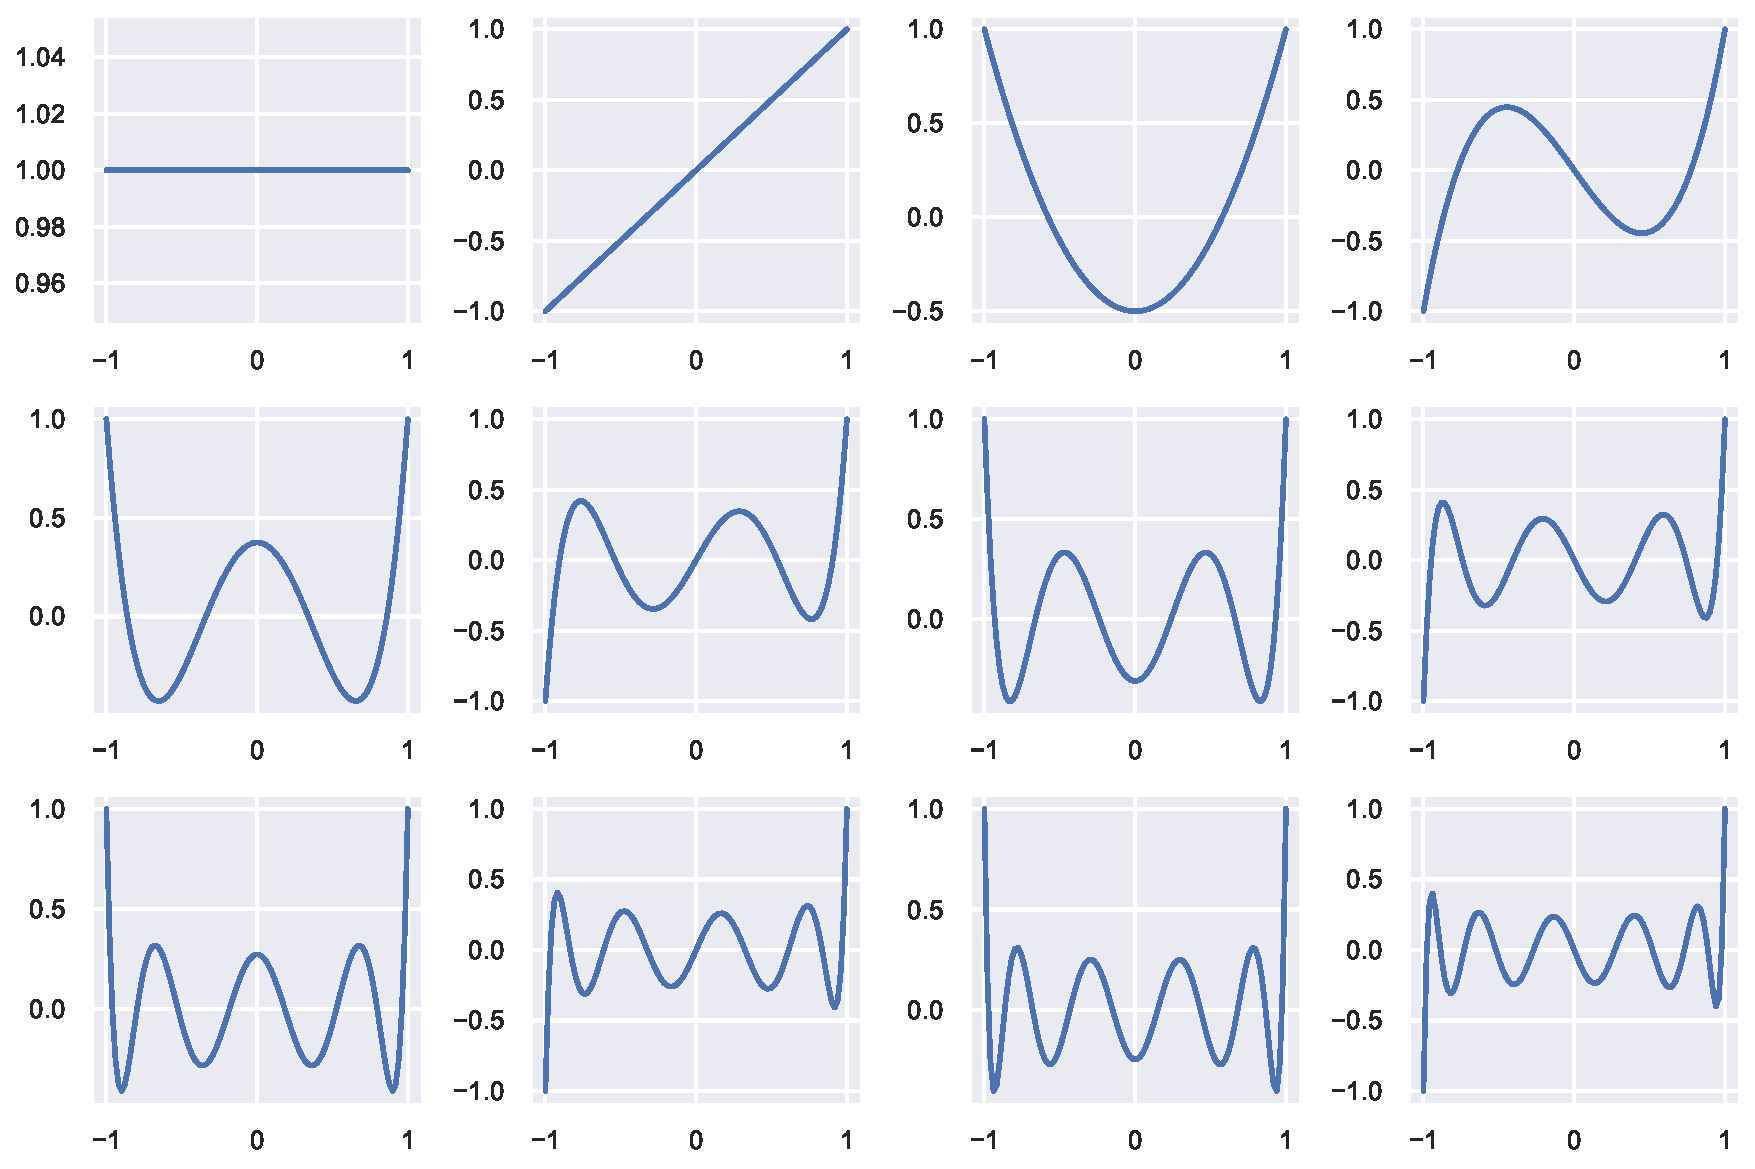
\includegraphics[height=\paperheight]{figures/legendre-polynomials}
\end{frame}

\begin{frame}{Associated Legendre Polynomials}
	\begin{lemma}
		For \(x \in [-1, 1]\) the polynomials
		\[
  		P_{m, n} (x) = \left( 1 - x^2 \right)^{m/2} \frac{d^{m}}{dx^{m}} P_n (x)
		\]
		solve the associated Legendre differential equation.
	\end{lemma}
	
	\begin{alertblock}{Observation}<2->
		If \(m > n\) then \(P_{m, n}(x) = 0\) for all \(x\).
	\end{alertblock}
\end{frame}

\begin{frame}
	\centering
	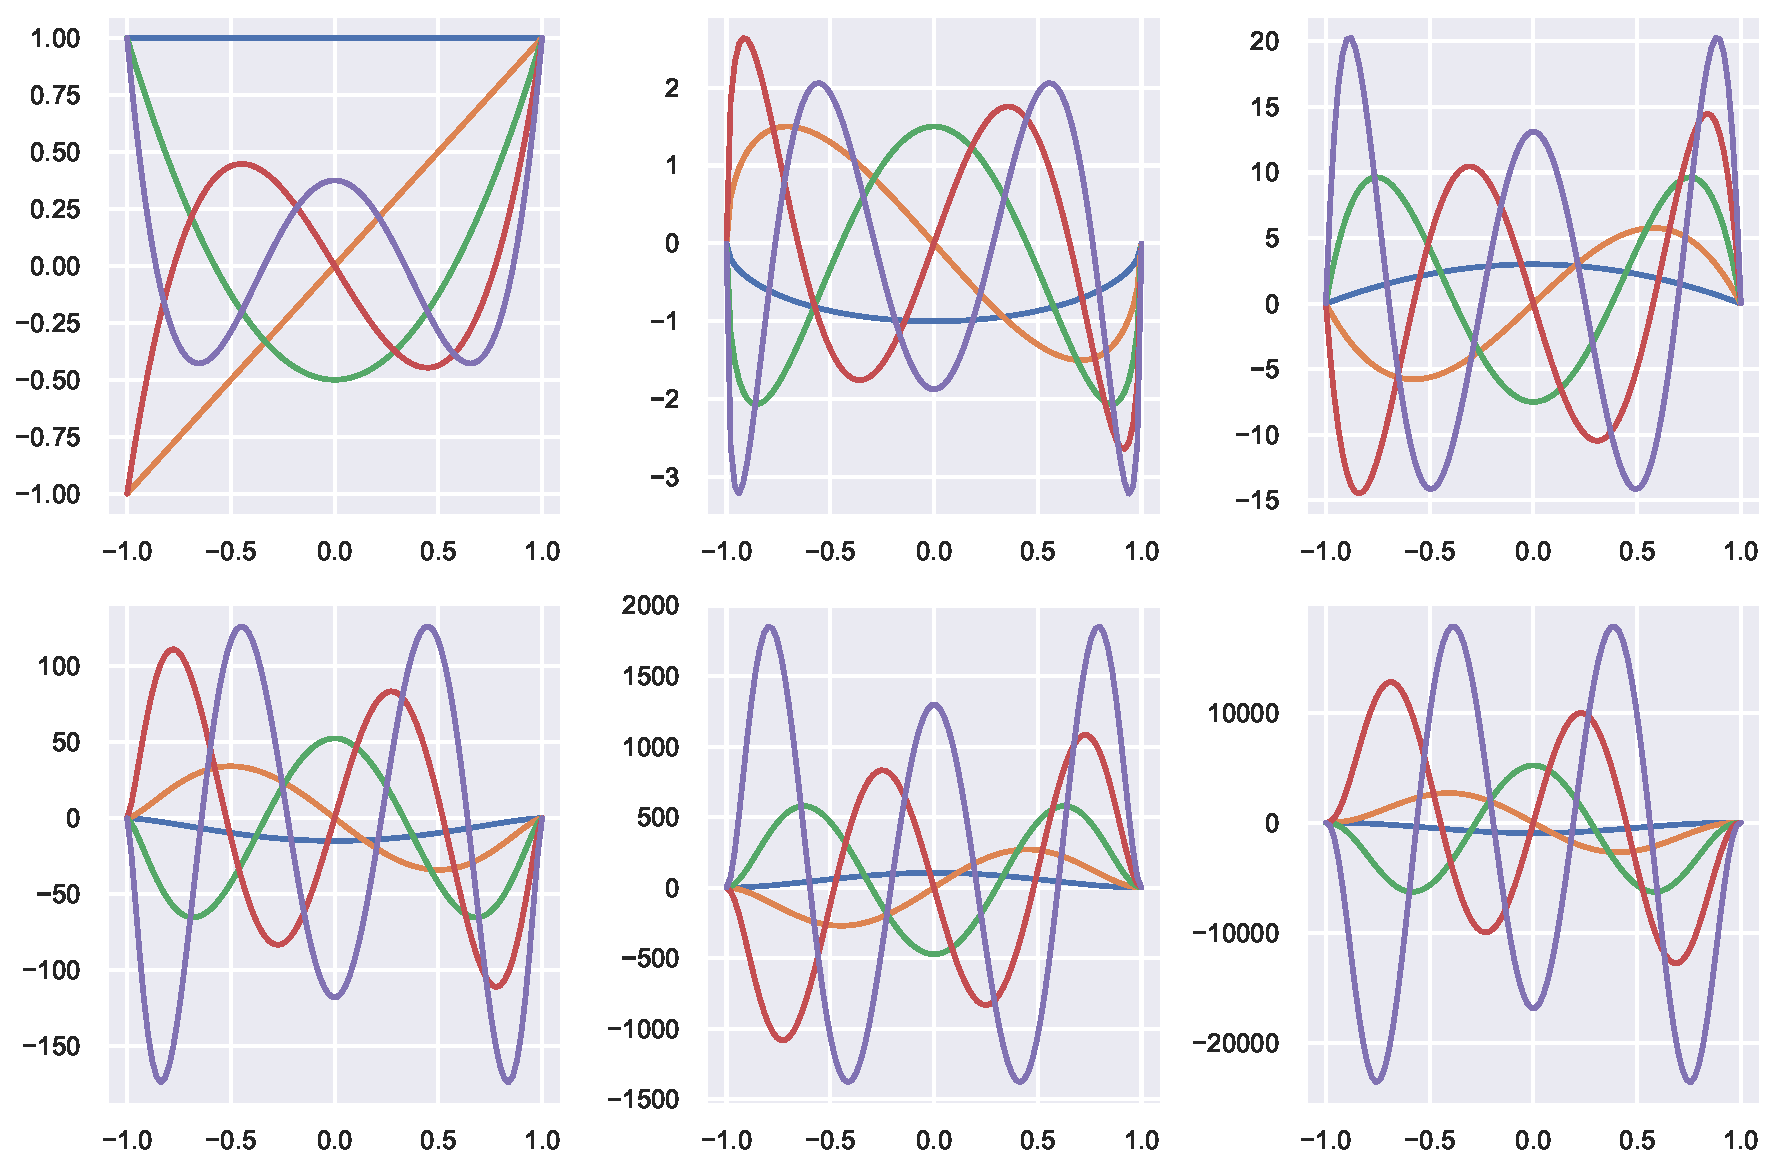
\includegraphics[height=\paperheight]{figures/associated-legendre-polynomials}
\end{frame}


\begin{frame}{Putting it back together}
	\begin{block}{The Problem}
		\[
			\nabla^2_s f(\varphi, \vartheta) = \lambda f(\varphi, \vartheta)
		\]
	\end{block}
	\begin{alertblock}{Current solution}
  	\[
			\tilde{Y}_{m, n}(\varphi, \vartheta)
				= \Phi(\varphi) \Theta(\vartheta)
				= e^{im\varphi} P_{m, n}(\cos\vartheta)
  	\]
	\end{alertblock}
	\begin{block}{Conditions}<2->
		\(m, n \in \mathbb{Z}\) and \(m < n\)
	\end{block}
\end{frame}

\bgroup
\setbeamercolor{background canvas}{bg=black}
\setbeamertemplate{navigation symbols}{}
\begin{frame}{Intuition for why \(m\) and \(n\) are Integers}
\end{frame}
\egroup

%\begin{frame}{What do they look like?}
%	\begin{center}
		% 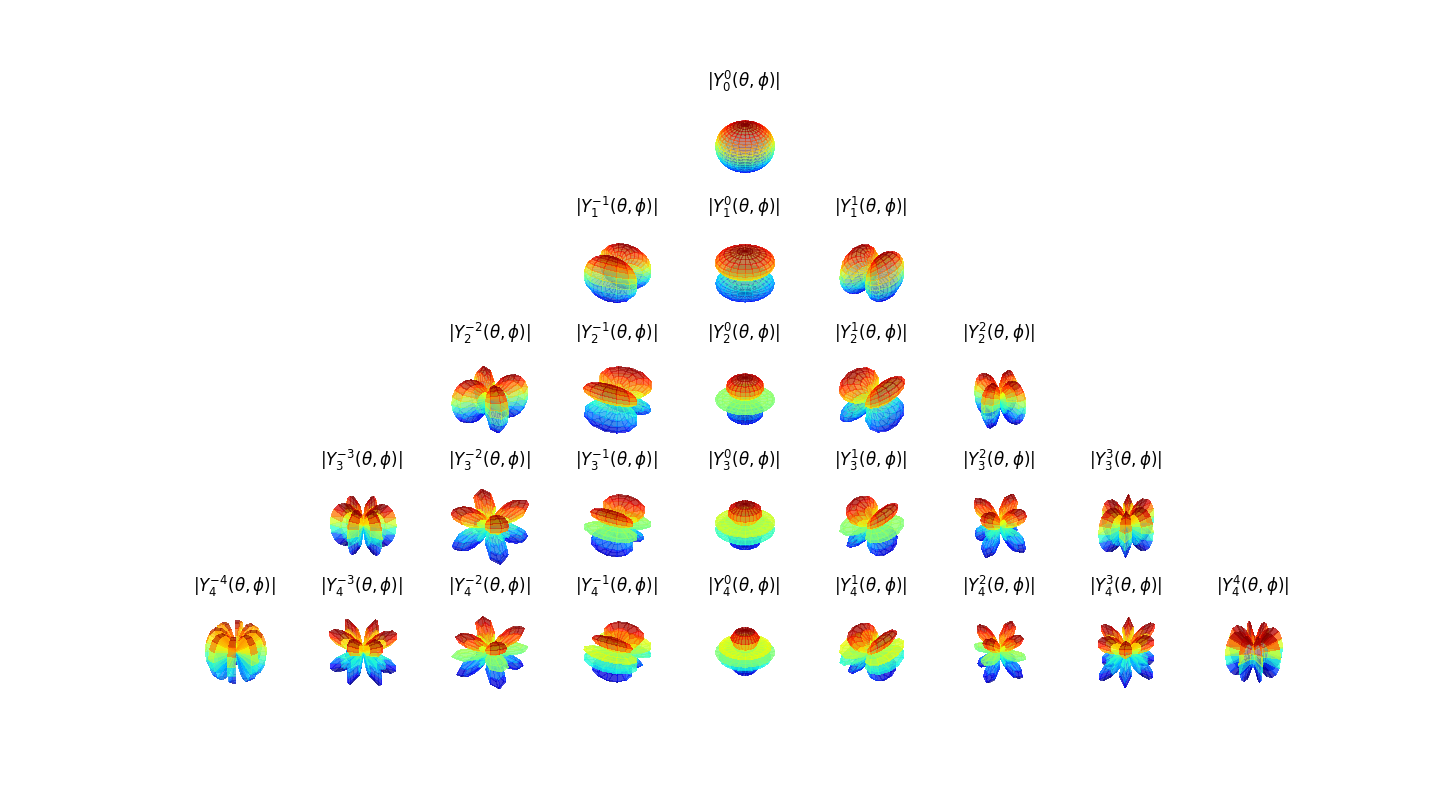
\includegraphics[height=.9\paperheight, clip, trim=100 10 100 10]{figures/spherical-harmonics-triangle}
%	\end{center}
%\end{frame}

\frame{
	\centering \noindent
	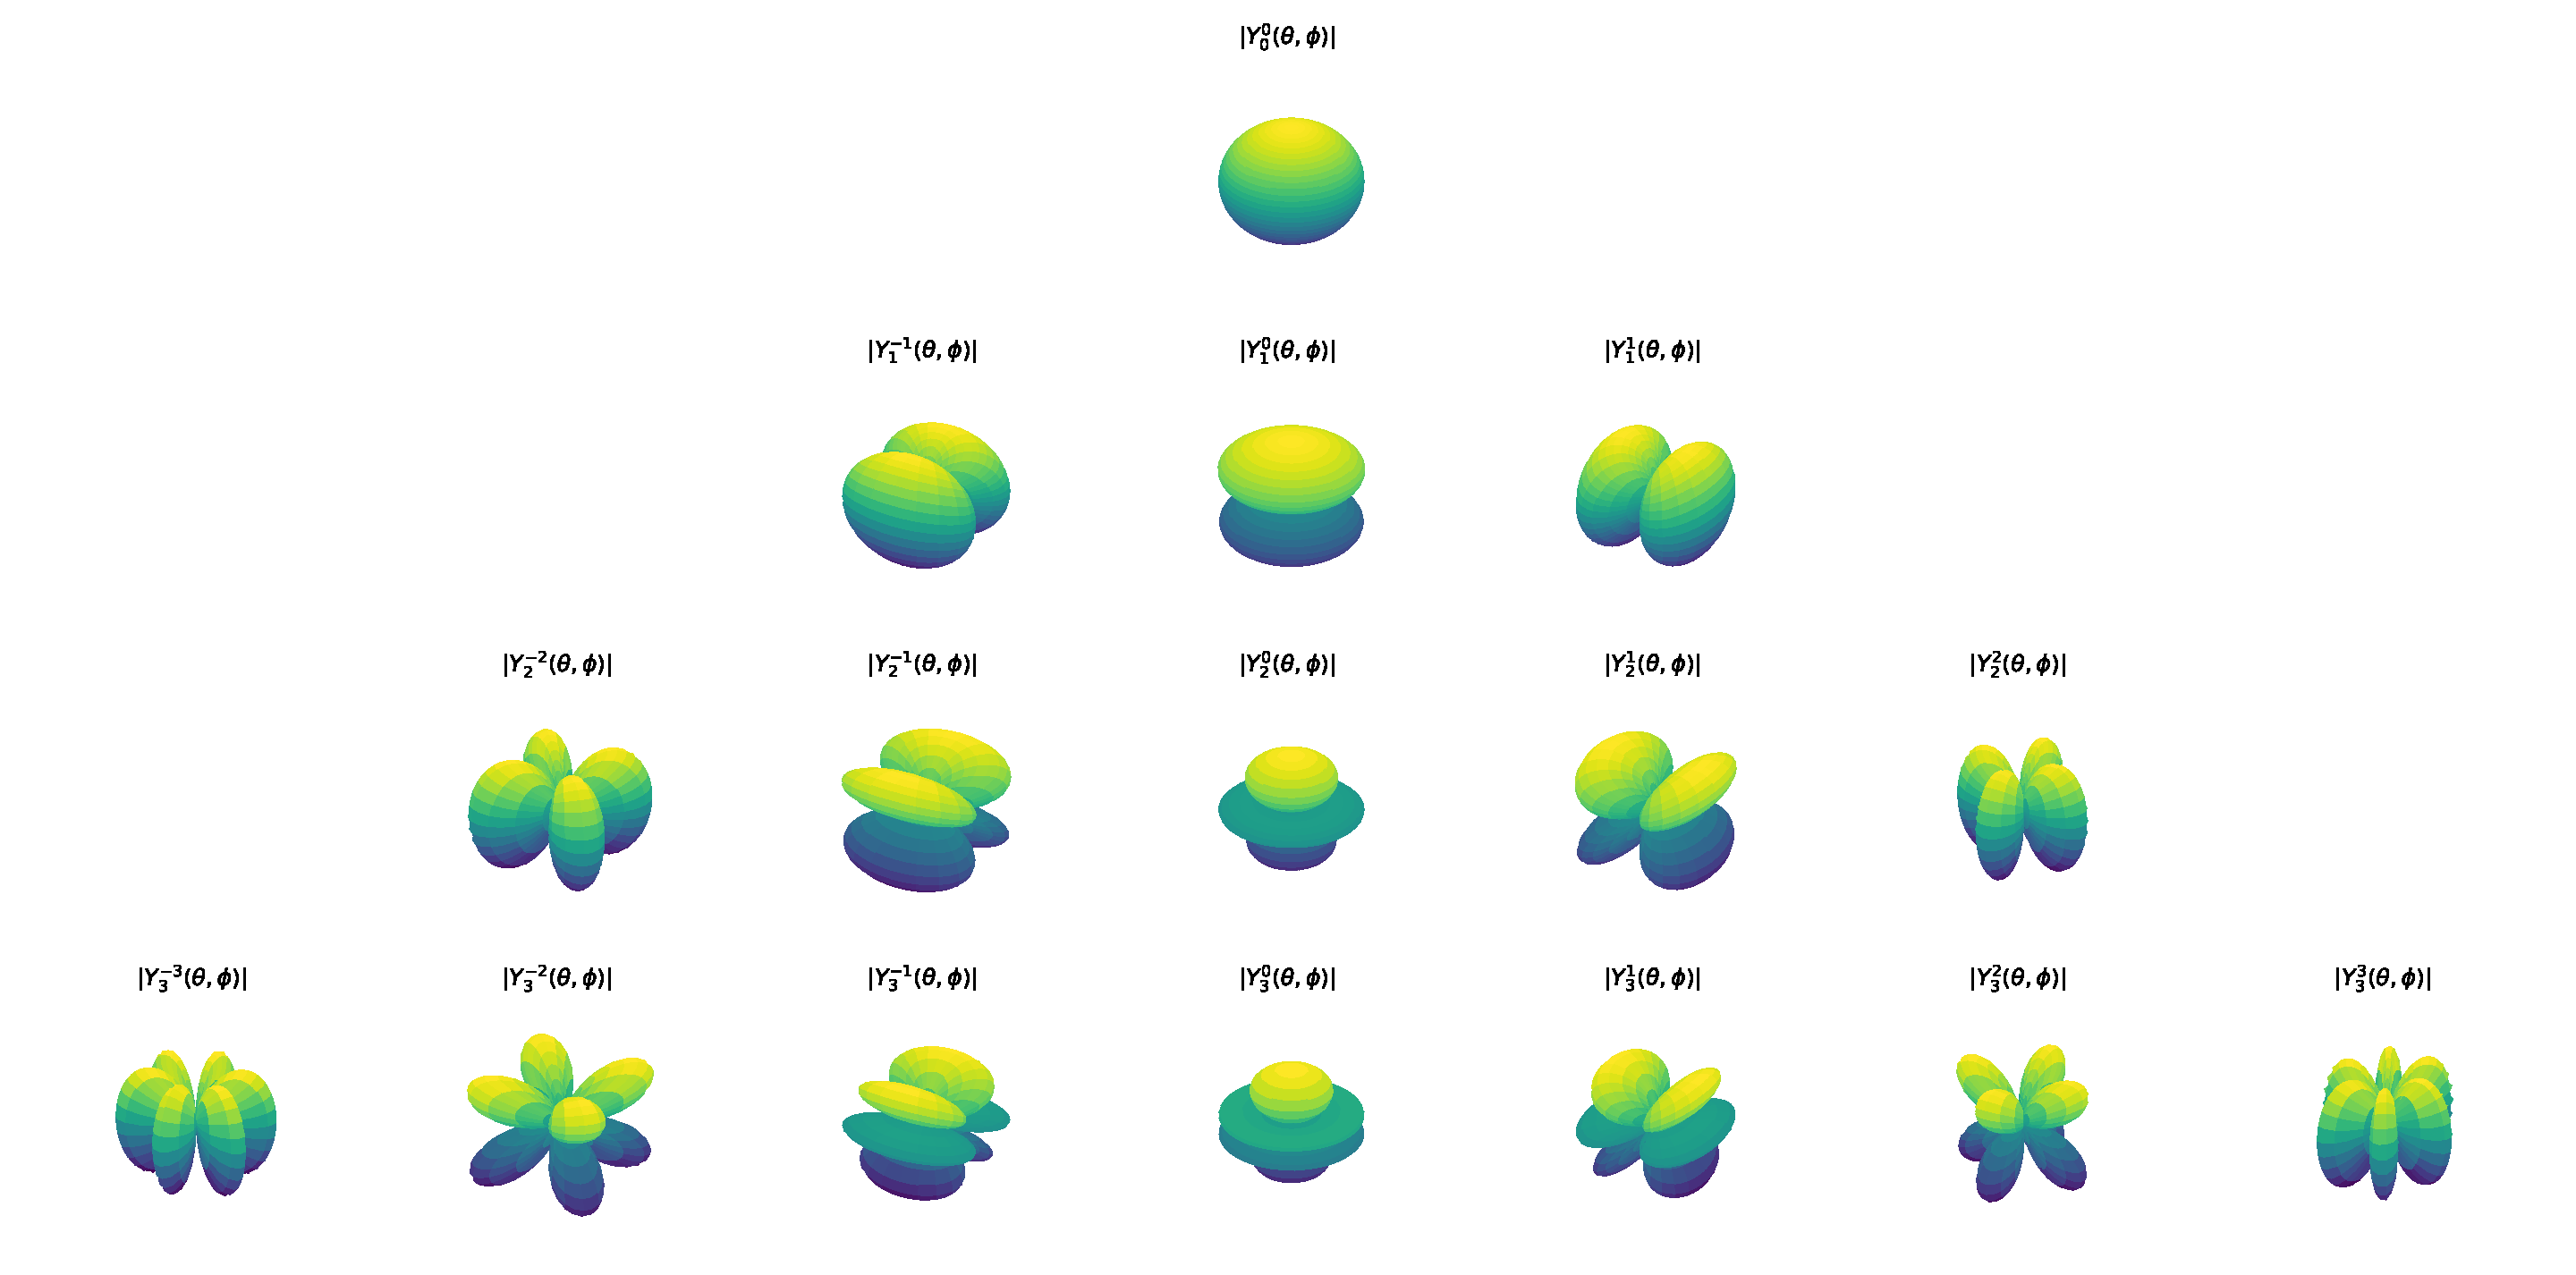
\includegraphics[height=.8\paperheight, clip, trim=50 0 0 0]{figures/spherical-harmonics-triangle-new}
}

\begin{frame}{Research Question}
	\begin{block}{Recurrence Relation(s)?}
		\begin{align*}
			\tilde{Y}_{m+1, n} &\stackrel{?}{=} f(\tilde{Y}_{m, n}, \tilde{Y}_{m-1, n}, \tilde{Y}_{m, n-1}, \ldots) \\
			\tilde{Y}_{m, n+1} &\stackrel{?}{=} f(\tilde{Y}_{m, n}, \tilde{Y}_{m-1, n}, \tilde{Y}_{m, n-1}, \ldots) \\
			\tilde{Y}_{m+1, n+1} &\stackrel{?}{=} f(\tilde{Y}_{m, n}, \tilde{Y}_{m-1, n}, \tilde{Y}_{m, n-1}, \ldots)
		\end{align*}
	\end{block}
\end{frame}

\section{Fourier on \(S^2\)}

\begin{frame}{Basis functions?}
	The functions \(\tilde{Y}_{m, n}\) span the space of nice functions \(S^2 \to \mathbb{C}\).
	
	\begin{definition}<2->
		The inner product of nice functions \(f(\varphi, \vartheta)\) and \(g(\varphi, \vartheta)\) from \(S^2\) to \(\mathbb{C}\) is
		\[
			\langle f, g \rangle
				= \iint_{S^2} f(\varphi, \vartheta) \overline{g}(\varphi, \vartheta) \, d\Omega
				\uncover<3->{
  				= \int\limits_0^{2\pi} \int\limits_0^{\pi}
  					f(\varphi, \vartheta) \overline{g}(\varphi, \vartheta)
  					\sin\vartheta \, d\vartheta d\varphi
				}
		\]
	\end{definition}
\end{frame}

\begin{frame}{Orthonormality}
	\begin{definition}<1->
		A set of basis functions are \emph{orthonormal} if
		\[
			\langle B_{m, n}, B_{m', n'} \rangle = \begin{cases}
				1 & m = m' \wedge n = n' \\
				0 & \text{otherwise}
			\end{cases}
		\]
	\end{definition}

	\begin{alertblock}{Problem}<2->
  	\[
  		\langle \tilde{Y}_{m, n}, \tilde{Y}_{m', n'} \rangle = \begin{cases} \displaystyle
  			\frac{4 \pi}{2n+1} \frac{(n+m)!}{(n-m)!} &  m = m' \wedge n = n' \\
  			0 & \text{otherwise}
  		\end{cases}
  	\]
	\end{alertblock}
\end{frame}

\begin{frame}{Spherical Harmonics}
	\begin{definition}<1->
		The orthonormal spherical harmonics are
		\[
			Y_{m, n}(\varphi, \vartheta) = N_{m, n} e^{im\varphi} P_{m, n}(\cos\vartheta)
		\]
		where the normalisation constant
		% FIXME: (-1)^m
		\[
			N_{m, n} = \sqrt{\frac{2n+1}{4 \pi} \frac{(n-m)!}{(n+m)!}}
		\]
	\end{definition}
	\begin{alertblock}{Fixed}<1->
		\[
			\langle Y_{m, n}, Y_{m', n'} \rangle = \begin{cases}
				1 & m = m' \wedge n = n' \\
				0 & \text{otherwise}
			\end{cases}
		\]
	\end{alertblock}
\end{frame}

\begin{frame}{Fourier Series}
	\begin{theorem}
		For nice periodic functions on \(S^2\):
  	\[
  		f(\varphi, \vartheta) = \sum_{m \in \mathbb{Z}} \sum_{n \in \mathbb{Z}}
				c_{m, n} Y_{m, n} (\varphi, \vartheta)
  	\]
		where
		\[
			c_{m, n} = \langle f, Y_{m, n} \rangle.
		\]
	\end{theorem}
\end{frame}

\begin{frame}{Fourier Expansion on \(S^2\)}
	\centering
	{\LARGE \bfseries Python Script} \\[1em]
	{(glorified pseudocode)}
	
	 	\[
  		f(\varphi, \vartheta) = \sum_{m} \sum_{n}
				c_{m, n} Y_{m, n} (\varphi, \vartheta)
  	\]
\end{frame}

\section{Quantum Mechanics}

\begin{frame}{Linear and Rotational Kinetic Energy}
	\begin{columns}
		\begin{column}{.5\linewidth}
			\begin{block}{Momentum and KE}<1->
				\[
					\vec{p} = m \vec{v},
					\quad
					E_k = \frac{\vec{p}^2}{2m}
				\]
			\end{block}
			\begin{alertblock}{QM Formulation}<3->
  			\[
						\vec{\hat{p}} = -i\hbar \bm{\nabla},
						\quad
						\hat{E}_k = -\frac{\hbar^2}{2m} \nabla^2
  			\]
			\end{alertblock}
		\end{column}
		\begin{column}{.5\linewidth}<2->
				\begin{block}{Angular Momentum and KE}
				\[
					\vec{L} = \vec{r}\bm{\times}{\vec{p}},
					\quad
					E_{k, a} = \frac{\vec{L}^2}{2m r^2}
				\]
			\end{block}
			\begin{alertblock}{QM Formulation}<4->
				Pretty long derivation yields:
				\begin{align*}
					% \hat{L}_z &= -i \hbar \frac{\partial}{\partial \varphi}, \\[1em]
					\hat{E}_{k, a} &= -\frac{\hbar^2}{2mr^2} \nabla^2_s
				\end{align*}
			\end{alertblock}
		\end{column}
	\end{columns}
\end{frame}

\iffalse
\begin{frame}{Intuition for the Operators}
	\begin{columns}
		\begin{column}{.5\linewidth}
			\begin{block}{Plane wave}<1->
				\[
					\Psi(\vec{x}, t) = \exp i(\vec{k} \bm{\cdot} \vec{x} + \omega t )
				\]
			\end{block}
			\begin{block}{Spatial derivative}<2->
				\begin{align*}
					\uncover<2->{
  					\bm{\nabla} \Psi(\vec{x}, t) &= 
  						\bm{\nabla} \exp i(\vec{k} \bm{\cdot} \vec{x} + \omega t ) \\
					}
					\uncover<3->{
						&= ik \exp i(\vec{k} \bm{\cdot} \vec{x} + \omega t ) \\
						&= ik \Psi(\vec{x}, t)
					}
				\end{align*}
			\end{block}
		\end{column}
		\begin{column}{.5\linewidth}
		\end{column}
	\end{columns}
\end{frame}
\fi

\bgroup
\setbeamercolor{background canvas}{bg=black}
\setbeamertemplate{navigation symbols}{}
\begin{frame}{Intuition for the Operators}
\end{frame}
\egroup

\begin{frame}{Schrödinger Equation}
	\begin{block}{Time independent SE}
		\[
			% hamiltonina
			\only<1>{
				\mathrm{\hat{\mathcal{H}}} | \Psi \rangle = E | \Psi \rangle
			}
			% KE + U
			\only<2>{
				\left(
					\hat{E}_k + U
				\right) | \Psi \rangle = E | \Psi \rangle
			}
			% KE with p
			\only<3>{
				\left(
					\frac{\vec{\hat{p}}^2}{2m} + U
				\right) | \Psi \rangle = E | \Psi \rangle
			}
			% KE with p as 1D derivative
			\only<4>{
				\text{Meili} \qquad
				\left[
					- \frac{\hbar^2}{2m} \frac{d^2}{d x^2} + U(x)
				\right] \Psi(x) = E \Psi(x)
			}
			% KE with p as 3D derivative
			\only<5>{
				\text{3D} \qquad
				\left[
					- \frac{\hbar^2}{2m} \nabla^2 + U(\vec{x})
				\right] \Psi(\vec{x}) = E \Psi(\vec{x})
			}
			% Decompose laplacian
			\only<6-7>{
				\left\{
					- \frac{\hbar^2}{2m} \frac{1}{r^2} \left[
						\nabla^2_s - \frac{\partial}{\partial r} \left(
							r^2 \frac{\partial}{\partial r}
						\right)
					\right] + U(\vec{r})
				\right\} \Psi(\vec{r}) = E \Psi(\vec{r})
			}
			% rewrite using L
			\only<8>{
				\left[
					\frac{\vec{\hat{L}}^2}{2mr^2}
					+ \frac{1}{r^2} \frac{\partial}{\partial r} \left(
							r^2 \frac{\partial}{\partial r}
						\right)
					+ U(\vec{r})
				\right] \Psi(\vec{r}) = E \Psi(\vec{r})
			}
			% rewrite using E_ka
			\only<9>{
				\left[
					\hat{E}_{k,a}
					+ \frac{1}{r^2} \frac{\partial}{\partial r} \left(
							r^2 \frac{\partial}{\partial r}
						\right)
					+ U(\vec{r})
				\right] \Psi(\vec{r}) = E \Psi(\vec{r})
			}
			% What is KE
			\only<10>{
				\Bigg[
					\underbrace{\hat{E}_{k,a}
					+ \frac{1}{r^2} \frac{\partial}{\partial r} \left(
							r^2 \frac{\partial}{\partial r}
						\right)}_\text{Kinetic Energy}
					+\, U(\vec{r})
				\Bigg] \Psi(\vec{r}) = E \Psi(\vec{r})
			}
			% Introduce E_kr
			\only<11>{
				\Bigg[
					\hat{E}_{k,a}
					+ \underbrace{\frac{1}{r^2} \frac{\partial}{\partial r} \left(
							r^2 \frac{\partial}{\partial r}
						\right)}_{\text{Radial KE } \hat{E}_{k, r}}
					+ U(\vec{r})
				\Bigg] \Psi(\vec{r}) = E \Psi(\vec{r})
			}
			\only<12->{
				\left\{
					\hat{E}_{k,a} + \hat{E}_{k,r} + U(\vec{r})
				\right\} \Psi(\vec{r}) = E \Psi(\vec{r})
			}
		\]
	\end{block}
	\only<6>{
  	\begin{columns}
  		\begin{column}{.6\linewidth}
  			\Large
  			\textit{But why?} \\[2em]
  
  			{\bfseries Hydrogen atom has radial symmetry!}
  		\end{column}
  		\begin{column}{.35\linewidth}
      	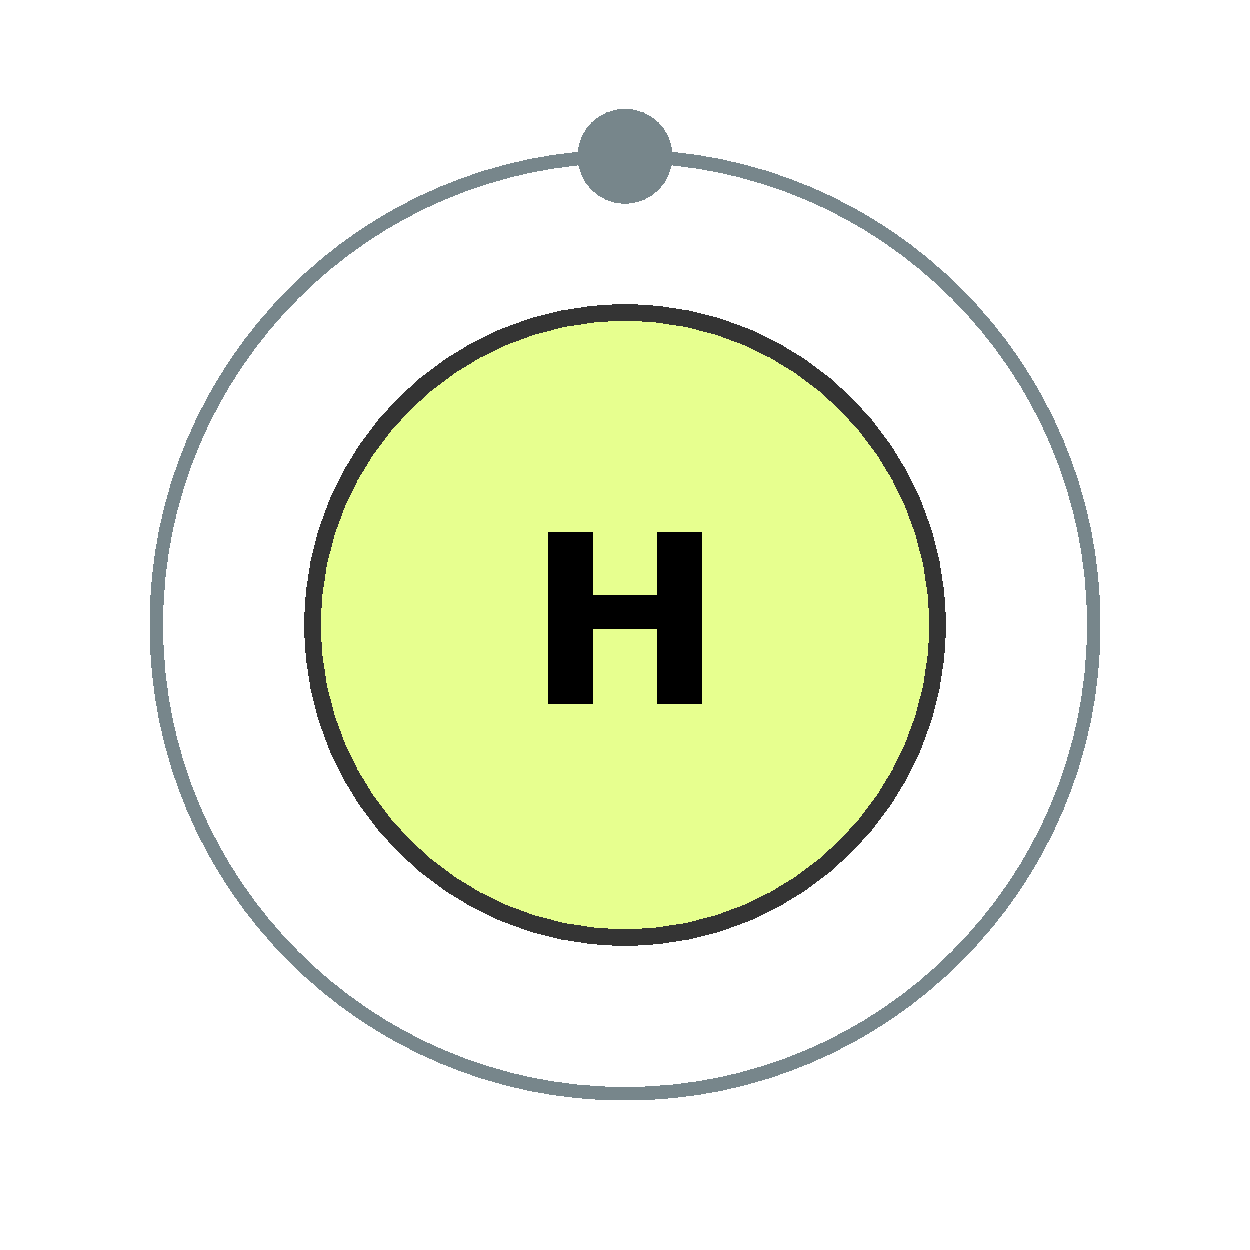
\includegraphics[width=\linewidth]{figures/hydrogen}
  			\nocite{depiep_electron_2013}
  		\end{column}
  	\end{columns}
	}

	\begin{alertblock}{Eigenvalue Problem}<13->
		\[
			\hat{E}_{k,a} \Psi(\varphi, \vartheta) = E \Psi(\varphi, \vartheta)
		\]
	\end{alertblock}
\end{frame}

\begin{frame}{Electron Orbitals\footnote{Only the angular component}}
	
	\begin{columns}
		\begin{column}{.5\linewidth}
    	\begin{block}{Eigenvalue Problem}
    		\only<1>{
      		\[
      			\hat{E}_{k,a} \Psi(\varphi, \vartheta) = E \Psi(\varphi, \vartheta)
      		\]
    		}
    		\only<2->{
    			\[
      			-\frac{\hbar^2}{2m} \nabla^2_s \Psi(\varphi, \vartheta) = E \Psi(\varphi, \vartheta)
      		\]
    		}
    	\end{block}
			\begin{alertblock}{Solutions}<3->
				\[
					\Psi(\varphi, \vartheta) = Y_{m, n} (\varphi, \vartheta)
				\]				
			\end{alertblock}
		\end{column}
		\begin{column}{.5\linewidth}
			\begin{tikzpicture}
      	\uncover<3->{
    			\node (i1) {
          	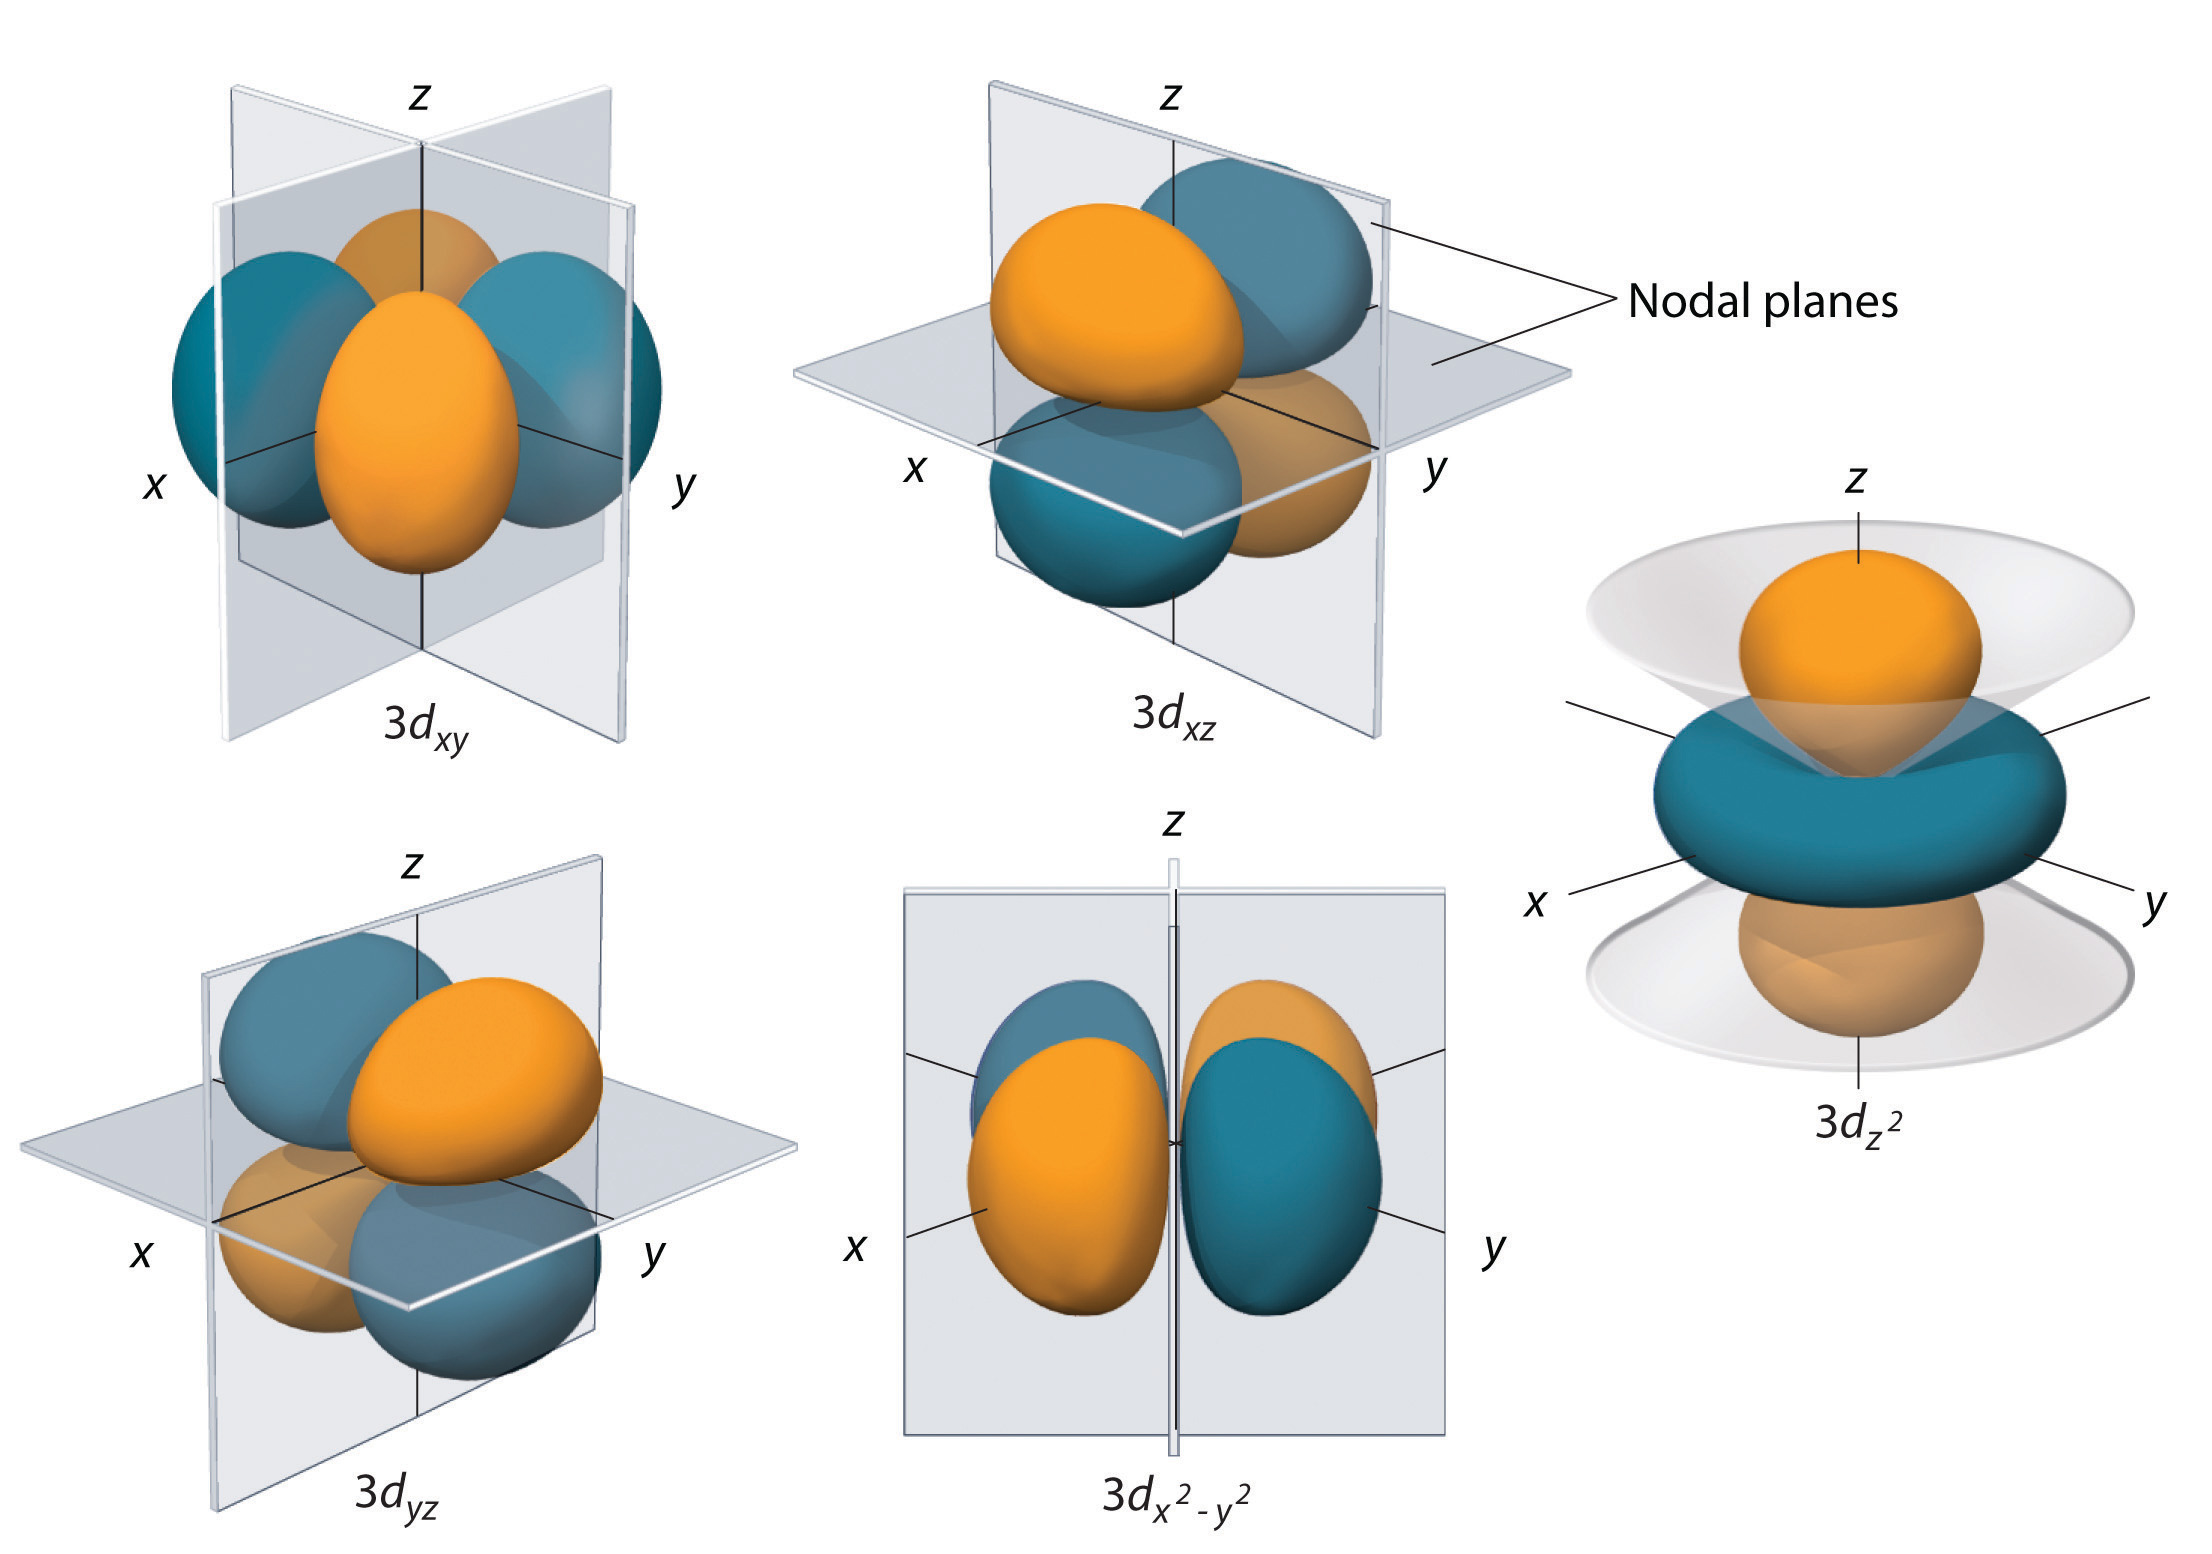
\includegraphics[width=\linewidth]{figures/electron-orbitals}
    			};
      	}
      	\uncover<4->{
      		\node (i2) at ($(i1) + (0, 0)$) {
    				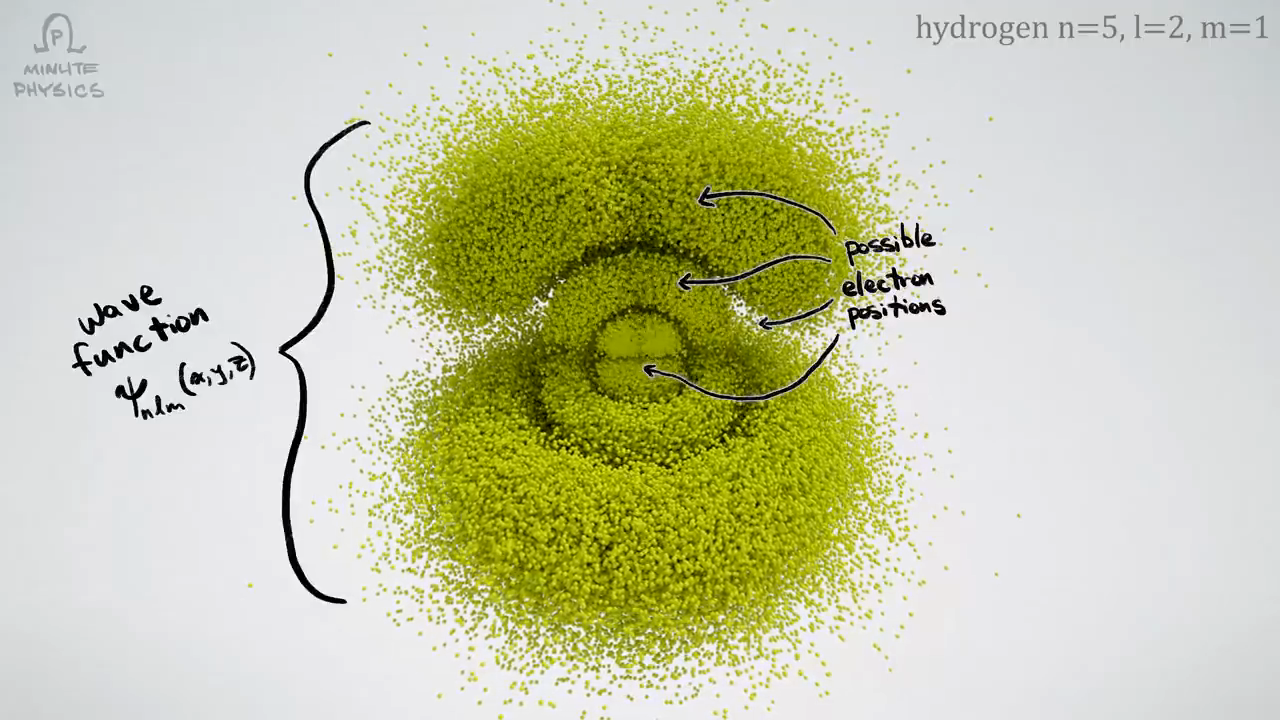
\includegraphics[width=\linewidth]{figures/orbitals-minutephysics}
      		};
      	}
    	\end{tikzpicture}
			
			\begin{exampleblock}{Radial component}<4->
				We can leave that for another day.
			\end{exampleblock}
		\end{column}
	\end{columns}
\end{frame}

\frame{
	\centering
	{\LARGE It was a lot, but I'm sure you got all of that.} \\[3em]
	{\LARGE \bfseries Questions?}
}

\begin{frame}{Bibliography}
	\renewcommand*{\bibfont}{\tiny}
	\printbibliography
\end{frame}

\end{document}

% vim:et:ts=2:sw=2:wrap:nolinebreak:
